% ------------------------------------------------------------------------
%
% -------------------      Plantilla_UIS.tex       -----------------------
%               ESTE ES EL MAIN.TEX ESTE ARCHIVO LLAMA A TODOS LOS ARCHIVOS QUE COMPONEN LA TESIS....
% ------------------------------------------------------------------------
% ------------------------------------------------------------------------
% ------------------------------------------------------------------------
% Versión de plantilla para realización de informes de trabajo de grado
% construida para uso de la Universidad Industrial de Santander.
%
% Reservados todos los derechos
%
% Bucaramanga, Colombia
%
% Febrero 03 de 2019
%
% ------------------------------------------------------------------------
% ------------------------------------------------------------------------
% ------------------------------------------------------------------------
%
% ------------------------------------------------------------------------
\documentclass[letter,oneside,12pt,spanish]{report}          % Encabezados
% ------------------------------------------------------------------------
\usepackage{uislatexstyleAPA}                           % Libreria UIS APA
% ------------------------------------------------------------------------
% Ingrese en este punto las librerías específicas de usuario
% ------------------------------------------------------------------------
\usepackage{epsfig}
\usepackage{amsmath}
\usepackage{amssymb}
\usepackage{subfigure}
% ------------------------- NUEVO-----------------------------------------------
\bibliography{xbib.bib}
% ------------------------------------------------------------------------
\begin{document}                                     % Inicio de documento
% ------------------------------------------------------------------------
% Definición silábica de palabras
% ------------------------------------------------------------------------
%\hyphenation{pro-por-cio-nal di-se-ño}
% ------------------------------------------------------------------------
% Titulo resumido del trabajo que aparecerá en cornisa
% ------------------------------------------------------------------------
\title{Caracterización de perfiles atmosféricos para la colaboración LAGO}
% ------------------------------------------------------------------------
% Elementos previos al contenido del trabajo
% ------------------------------------------------------------------------
% ------------------------------------------------------------------------
%                               Portadilla
% ------------------------------------------------------------------------

\begin{center}

Caracterización de perfiles atmosféricos para la cadena de simulación de la colaboración LAGO \vspace{1.5cm}

Jennifer Grisales Casadiegos\\ \vspace{1.5cm}

Trabajo de Grado para optar al título de Física\\ \vspace{1.5cm}

Director\\
Luis A. Núñez\\
Doctorado en Ciencias\\ \vspace{1cm}
Co-Director\\
Christian Sarmiento Cano\\
Maestría en Física \vspace{1.5cm}

Universidad Industrial de Santander\\
Facultad de Ciencias\\
Escuela de Física\\
Bucaramanga\\
2020\\

\end{center}

% ------------------------------------------------------------------------
%                             Nota de proyecto
% ------------------------------------------------------------------------

\newpage

\begin{figure}[htb!]
\centering
\includegraphics[width=1.0\textwidth]{Secs/NOTA_TESIS.pdf}
\end{figure}

% ------------------------------------------------------------------------
%                             Autorización
% ------------------------------------------------------------------------

\newpage


\begin{figure}[htb!]
\centering
\includegraphics[width=1\textwidth]{Secs/Carta_AUTORIZACIÓN.pdf}
\end{figure}

% ------------------------------------------------------------------------ 
             % Portadilla, formato de nota y autorización
% ------------------------------------------------------------------------
% \addcontentsline{toc}{chapter}{Dedicatoria}
  
%   \cleardoublepage
\newpage

\vspace*{\stretch{3}}

\begin{flushleft}
\textit{¿En perseguirme, mundo, qué interesas?}\newline
\textit{¿En qué te ofendo, cuando sólo intento}\newline
\textit{poner bellezas en mi entendimiento}\newline
\textit{y no mi entendimiento en las bellezas?}\newline
\textit{Yo no estimo tesoros ni riquezas,}\newline
\textit{y así, siempre me causa más contento}\newline
\textit{poner riquezas en mi entendimiento}\newline
\textit{que no mi entendimiento en las riquezas.}\newline
\textit{Y no estimo hermosura que vencida}\newline
\textit{es despojo civil de las edades}\newline
\textit{ni riqueza me agrada fementida,}\newline
\textit{teniendo por mejor en mis verdades}\newline
\textit{consumir vanidades de la vida}\newline
\textit{que consumir la vida en vanidades.}\newline
\textit{``Quéjase de la suerte" por Juana Inés de Asbaje.}\newline

\textit{Este trabajo va dedicado a todas las mujeres que han defendido nuestro derecho al conocimiento.}
\end{flushleft}



\clearpage                                   % Dedicatoria
% ------------------------------------------------------------------------
%\addcontentsline{toc}{chapter}{Agradecimientos}
\newpage
\chapter*{Agradecimientos}

Son muchas las personas que, sabiéndolo o no, fueron contribuciones significativas, en una combinación lineal que determinó el camino de mi formación como Física. A todos y todas, gracias. Fuertemente en mis recuerdos mis compañeros de aprendizaje Edwin Florez, Genderson Rueda y Yerson Barragán, con quienes pese a las dificultades, disfrutamos esta etapa universitaria formando no solo nuestro pensamiento científico, sino también construyendo una necesaria conciencia de clase que orientará nuestro quehacer académico y político por siempre. Debo agradecer a mi madre y mi padre, porque debido a su formación, desde mi infancia nació el sueño de vivir la ciencia. Personas como José Quintero que me alentaron a seguir adelante y sacar valentía de donde no había, gracias. También a Jesús Sánchez por abrirme las puertas de su casa, y su familia, gracias por todo el afecto y el apoyo incondicional. A mi mejor amiga Luz Marina Cabrera por ser mi confidente y por jugar conmigo a dibujarnos mutuamente alas para volar y soñar.

Gracias a Luis Núñez por inspirarme siempre y mostrarme que la ciencia es el camino. Gracias Christian Sarmiento por creer en mí y por su tiempo que valoré infinitamente. También gracias a Yeinzon Rodríguez porque me demostró que es posible seguir viendo la física con curiosidad y pasión.

Finalmente quiero agradecer a Jesús Peña haber sido mi apoyo emocional en todo este proceso. Por ser mi ejemplo e inspiración de esfuerzo, perseverancia, trabajo duro y amor genuino por la ciencia. Gracias por tanto amor.                           % Agradecimientos
% ------------------------------------------------------------------------
\tableofcontents                                      % Tabla de contenido
% ------------------------------------------------------------------------
\listoffigures                         % Lista de figuras, tablas y anexos
\listoftables
\listofanexo
% ------------------------------------------------------------------------
%\include{Secs/glosario}                             % Glosario de términos
% ------------------------------------------------------------------------
% Contenido del Informe
% ------------------------------------------------------------------------
%\addcontentsline{toc}{chapter}{RESUMEN}
\newpage
\chapter*{Resumen}
\label{sec:resum}
\footnotesize{
\noindent\textbf{TÍTULO:} CARACTERIZACIÓN DE PERFILES ATMOSFÉRICOS PARA LA CADENA DE SIMULACIÓN DE LA COLABORACIÓN LAGO\astfootnote{Trabajo de grado}

\noindent\textbf{AUTORA:} Jennifer Grisales Casadiegos\asttfootnote{Facultad de Ciencias. Escuela de Física. Director: Luis A. Núñez. Codirector: Christian Sarmiento.}

\noindent\textbf{PALABRAS CLAVES: } Astropartículas, flujo de secundarios, atmósfera, simulaciones, cascadas aéreas extensas.

\noindent \textbf{DESCRIPCIÓN: } \\
Uno de los objetivos del programa de clima espacial del \textit{Latin American Giant Observatory} (LAGO), es estudiar la influencia de la actividad solar en las variaciones del flujo de partículas secundarias, producidas durante la interacción de las astropartículas con la atmósfera. Con este fin, se realiza una cadena de simulaciones, que estima de forma detallada, el desarrollo del primario desde su ingreso a la atmósfera terrestre, hasta la respuesta en los detectores Cherenkov de agua. El presente trabajo, completa esta cadena de simulaciones, concentrándose en el estudio del efecto que tiene la atmósfera en el flujo de fondo de secundarios. Para ello, se desarrolló una metodología que permite la creación y uso de perfiles atmosféricos mensuales, para cualquier ubicación geográfica, en las simulaciones de EAS dentro del código CORSIKA. Además se demostró la pertinencia de reemplazar los modelos atmosféricos predeterminados por nuevos perfiles, basados Sistema Global de Asimilación de datos (GDAS), comprobando, que los nuevos modelos atmosféricos mensuales, son capaces de reproducir, en el flujo de secundarios, el efecto de los cambios de temperatura a lo largo del año, y permitiendo refinar las estimaciones realizadas.
}\normalsize
\clearpage                                               % Resumen
%\addcontentsline{toc}{chapter}{Abstract}
\newpage
\chapter*{Abstract}
\label{sec:abst}
\footnotesize{
\noindent\textbf{TITLE:} CHARACTERIZATION OF ATMOSPHERIC PROFILES FOR THE LAGO SIMULATION CHAIN\astfootnote{Bachelor Thesis}

\noindent\textbf{AUTHOR:} Jennifer Grisales Casadiegos.\asttfootnote{Facultad de Ciencias. Escuela de Física. Director: Luis A. Núñez. Codirector: Christian Sarmiento.}

\noindent\textbf{KEYWORDS: } Astroparticle, particle flux, atmosphere, simulation, extensive air shower.

\noindent\textbf{DESCRIPTION:} One of the main objectives of the Space Weather program of the Latin American Giant Observatory (LAGO), is to study the influence of the solar activity on the secondary particle flux  variations, produced during the interaction between astroparticles with atmosphere. To this end, a chain of simulations is carried out, which estimates in detail, the Primary's development, from its entry into the Earth's atmosphere, to the Water Cherenkov Detector response. This work, complete the simulation chain, focusing their interest in to study the atmospheric effect on the secondary particle flux. To do this it developed a methodology that allows the creation and use of monthly atmospheric profiles, for any localization, in the EAS simulations within the CORSIKA code. Furthermore, the relevance to using the new monthly profiles it was checked, because they are able to reproduce in the secondary particle flux, the effect of the temperature changes along the year. This allows refine the estimates made.
}\normalsize
\clearpage                                              % Abstract
% ------------------------------------------------------------------------
% Capítulos
% ------------------------------------------------------------------------
\addcontentsline{toc}{chapter}{Introducción}
\newpage
\chapter*{Introducción}
\label{sec:intro}

\noindent El Sol es la estrella más cercana a la Tierra y la principal fuente de energía para la vida en nuestro planeta. Su actividad se manifiesta en forma de cambios en la luminosidad, campo magnético, viento solar y transporte de partículas, además que lo hace a diferentes ritmos, desde minutos hasta siglos  (\cite{Balogh_2008}). El periodo de actividad más conocido el el ciclo de 11 años que se caracteriza por el aumento y la disminución del número de manchas solares donde se concentra el campo magnético debido al mecanismo de convección de su plasma (\cite{Balogh_2008}).

El estudio exhaustivo de la dinámica solar y todos los fenómenos determinados por la interacción entre el viento solar, el campo magnético interplanetario y el campo magnético terrestre se conoce hoy como \textit{Clima Espacial} (\cite{singh_2021}). El término se empezó a usar en los años 50 y se popularizó en los años 90. Sin embargo, antes de eso ya se habían observado y caracterizado algunos fenómenos de clima espacial como las auroras, las tormentas magnéticas o los rayos cósmicos (\cite{cade_2015}). Por ejemplo, el primer registro de una tormenta magnética fue realizado por el naturalista Alexander von Humboldt en 1808 relacionándola con las manchas solares (\cite{Lakhina_2007}), o el registro en 1859 de la mayor tormenta magnética conocida \textit{el evento Carrington}, que causó auroras espectaculares y daños en las líneas telegráficas (\cite{hayakawa_2019}). En el siglo XX, el desarrollo de la tecnología espacial hizo que el clima espacial fuera más relevante, ya que podía afectar a los satélites, las comunicaciones, la navegación o la salud de los astronautas (\cite{Schrijver_2015}) y se comenzaron a desarrollar instrumentos tanto en el espacio como en la Tierra, que permiten observar el Sol, el viento solar, el campo magnético interplanetario, el campo magnético terrestre, la ionosfera y la atmósfera. 
%(\cite{cade_2015})

Entre estos instrumentos se encuentran los detectores de rayos cósmicos: partículas cargadas que provienen de diversas fuentes astrofísicas incluido el Sol, capaces de acelerar partículas a altas velocidades, abarcando un amplio espectro de energía (\cite{spurio_2015}).  No obstante, es un hecho bien establecido que al aumentar la energía, disminuye el número de partículas que pueden ser detectadas. En este contexto, el Sol y la galaxia se revelan como las fuentes predominantes, generando lo que hoy llamamos \textit{fondo de rayos cósmicos} (\cite{gaisser_2016}). Hasta la fecha, todas las observaciones realizadas han confirmado que los diversos fenómenos solares son la principal causa de alteración en este flujo de fondo, estableciendo así un vínculo directo entre la medición de estas partículas y la actividad solar (\cite{forbush_1954}).

Uno de los experimentos más importantes construidos para la medición indirecta de rayos cósmicos es el Observatorio Pierre Auger que se encuentra en la provincia de Mendoza, Argentina, y tiene como objetivo estudiar partículas de ultra alta energía (UHECR), es decir, aquellas con energías superiores a los $10^{18}eV$ (\cite{AugerGENERAL_2015}). Sin embargo, a partir del 2005 este observatorio implementó un sistema de detección adicional de baja energía denominado \textit{modo scaler} que registra el flujo de fondo en forma de número de partículas por segundo, con el objetivo de observar destellos de rayos gamma y eventos transitorios como Forbush Decreases (\cite{DASSO20121563}). Por lo tanto, este nuevo criterio de almacenamiento de eventos ha abierto un mundo de nuevos análisis e información física que en los últimos años ha logrado mayor interés en la comunidad científica.

La presente tesis de maestría hace parte de este conjunto de trabajos que busca caracterizar al arreglo de detectores de superficie como un sensor de alta resolución del rayos cósmicos galácticos (\cite{DASSO20121563}, \cite{asorey},\cite{masias_2017},\cite{Martin_Schimassek2022}). Mas específicamente, aquí presentamos un estudio de los efectos de la actividad solar a largo plazo sobre el flujo de rayos cósmicos secundarios en el Observatorio Pierre Auger, utilizando el modo Scaler, considerando el efecto que tienen los eventos transitorios en estas mediciones (\cite{roberta_2018}, \cite{Martin_Schimassek2022}). 

Para ello, se ha realizado un análisis de los datos del modo Scaler del Observatorio Pierre Auger, desde el año 2006 hasta el año 2021, y se han comparado con los datos de otros detectores y fuentes, como los monitores de neutrones, los satélites, las manchas solares y el campo magnético interplanetario. Se ha estudiado la correlación entre el flujo de rayos cósmicos y los parámetros solares, así como la respuesta del Observatorio a los eventos solares transitorios, como las erupciones solares y las eyecciones de masa coronal y su afectación al ciclo solar de 11 años.

%%%%%%%%%%%%
   % Introducción
%\include{Secs/T1}   % Objetivos
\newpage
%%%%%%%%%%%%%%%%%%%%%%%%%%%%----->SECCIÓN 2<-----%%%%%%%%%%%%%%%%%%%%%%%%%
\chapter{Rayos cósmicos}
%%%%%%%%%%%%%%%%%% NEWWWW
Los rayos cósmicos (CR) son partículas cargadas que viajan a través del espacio intergaláctico a velocidades cercanas a la luz. Estas partículas que provienen de diversas fuentes, incluyendo el Sol, supernovas, pulsares, agujeros negros entre otras, son en su mayoría protones y núcleos atómicos. Su composición es diversa, con una predominancia de protones $(89\%)$, seguidos por núcleos de helio $( 10\%)$ y núcleos pesados $( 1\%)$. También pueden estar constituidos por partículas elementales como electrones o fotones de alta energía  (\cite{kampert_2012}). 

En este capítulo, realizaremos una descripción de su origen y espectro de energías además de los mecanismos de detección utilizados en la actualidad, proporcionando una visión de cómo están siendo estudiados.  A continuación, exploraremos cómo se propagan a través de la heliósfera y el campo geomagnético para finalizar describiendo la morfología de las cascadas aéres extensas (EAS) producidas en la atmósfera terrestre y las interacciones hadrónicas y electromagnéticas que las generan. La comprensión de los fenómenos de interacción y decaimientos es esencial, ya que nuestro estudio se centra en la detección en tierra de la componente electromagnética de las EAS, especialmente los muones y electrones que llegan al nivel del suelo. 

\section{Origen y espectro de energías}

Los CR son en su mayoría hadrones, partículas subatómicas que incluyen protones y núcleos atómicos. Pueden tener energías de entre $10^{9}$ $eV$ hasta más allá de los $10^{20}$ $eV$. Aquellas con energías menores a $10^{15}$ $eV$ están sujetas grandes variaciones temporales, tanto periódicas como transitorias, debido a la influencia del Sol. Superior a esta energía los efectos heliosféricos se vuelven despreciables (\cite{spurio_2015}).
%  En el rango de baja energía, su detección está limitada por la existencia de un corte geomagnético, al menos en medidas realizadas cerca de la Tierra (\cite{Riggi_2023}).

Para su medición se pueden emplear diferentes métodos dependiendo de la energía del primario\footnote{En adelante llamaremos partículas primaria o \textit{primarios} a los CR que llegan a la tierra y no han interactuado con la atmósfera.}. Los métodos directos para la detección de CR implican el uso de instrumentos enviados al espacio en globos, cohetes o satélites para medir las características de las partículas que llegan a la Tierra (\cite{spurio_2015}). Algunos ejemplos de estos instrumentos incluyen los detectores de trazas nucleares, los espectrógrafos magnéticos, o los calorímetros, que calculan pérdida de energía (\cite{tomassetti_2023}).
%Un ejemplo representativo de un instrumento de detección directa es el Espectrómetro Magnético Alfa (AMS) en la Estación Espacial Internacional, que mide los rayos cósmicos de alta energía o el Espectrómetro de Isótopos de Rayos Cósmicos (CRIS) en la nave espacial Advanced Composition Explorer (ACE) (\cite{tomassetti_2023}), que proporciona mediciones de los isótopos de núcleos de GCR que van desde el helio hasta el zinc.

Los métodos indirectos de detección utilizan la atmósfera como calorímetro y detectan las partículas secundarias\footnote{En adelante llamaremos partículas secundarias o \textit{secundarios} a las partículas generadas por los procesos de interacción y decaimiento que se producen por la interacción de los CR primarios con la atmósfera.} producidas. Uno de los instrumentos más representativos para la detección indirecta es el Observatorio Pierre Auger, que utiliza múltiples técnicas para estudiar la física detrás de los CR de ultra alta energía a energías mucho más allá de las accesibles por los aceleradores de partículas (\cite{engel_2021}).

El espectro de energía de los CR caracterizado a través de una gran variedad de instrumentos, se puede observar en la figura \ref{fig:spectrum} en donde se observan 3 puntos de quiebre a diferentes valores de energía: la rodilla ($10^{15} eV$), la segunda rodilla ($10^{17}eV$) y el tobillo ($10^{19}eV$). Este espectro sigue una ley de potencia, del tipo $E^{-\gamma}$, con el exponente $\gamma$ en cada uno de estos quiebres (\cite{Riggi_2023}). Para visualizar mejor la tendencia del espectro, se suelen representar los valores de flujo multiplicados por $E^{\gamma}$, eligiendo un valor adecuado del exponente $\gamma$ (entre 2,5 y 3) como se observa en la figura \ref{fig:spectrum}. Esta representación permite verificar si la tendencia de los datos sigue esta ley, ya que idealmente los valores se dispondrían a lo largo de una línea horizontal.

\begin{figure}
    \centering
    \includegraphics[width=0.8\linewidth]{Figs/CR_spectrum.png}
    \caption{Espectro de energía de los CR primarios. Los puntos con diferentes colores y geometrías indican las mediciones realizadas por experimentos directos o indirectos. Fuente \cite{PDG}}
    \label{fig:spectrum}
\end{figure}

%%%%%%  ORIGEN DE LOS RAYOS CÓSMICOS DE ANTES DEL TOBILLO Y DESPUÉS DEL TOBILLO.
%%%% Pierre Cristofari (The transition From Galactic to Extragalactic cosmic rays)
Existe evidencia que sugiere que los CR con energías inferiores a la “rodilla” del espectro energético, tienen un origen galáctico modulado principalmente por el viento solar. Esta afirmación se basa en la observación de los rayos gamma emitidos por el disco galáctico pues se espera que la interacción de los CR con el material interestelar genere una señal de rayos gamma mejorada, es decir, un incremento en la emisión (\cite{Cristofari_2023}).

Por otro lado, cuando la energía de los CR supera un cierto umbral, conocido como el “tobillo”, se tiene evidencia de un origen extragaláctico (\cite{augerextra}). Esta transición se produce porque los CR de alta energía no pueden confinarse dentro de la galaxia cuando su radio de Larmor, que es el radio de la trayectoria en espiral que una partícula cargada sigue en un campo magnético, es mayor que el tamaño típico del halo galáctico (\cite{spurio_2015}). 
%Se tiene evidencia de que los CR de energías inferiores a la "rodilla" del espectro energético son de origen galáctico. Esto se basa en la observación de los rayos gamma del disco galáctico de los que se espera la emisión de una señal de rayos gamma mejorada (un incremento en la emisión) debido a la interacción de los CR con el material interestelar (\cite{Cristofari_2023}). Sin embargo, cuando la energía de los CR supera cierto umbral, conocido como el "tobillo", la fuente es de origen extragaláctico (\cite{augerextra}). Esta transición se debe a que los CR de alta energía no pueden confinarse dentro de la galaxia cuando su radio de Larmor es mayor que el tamaño típico del halo galáctico.
\section{Propagación de CR a través de la heliósfera}

Independientemente de su procedencia, todas las partículas primarias tienen que atravesar los campos magnéticos terrestre y solar para entrar en la atmósfera y es su energía la que determinará si tienen o no una interacción significativa. El examen minucioso de la composición y estructura del magnetismo solar ha permitido avanzar sustancialmente en nuestra comprensión del Sol y la forma como este modula los CR que viajan por el espacio interestelar. 

Son varias las capas que componen este cuerpo celeste, y cada una de ellas es esencial para la creación y distribución de su energía. En concreto, el interior, que incluye el núcleo y la zona radiativa constituye aproximadamente el $70\%$ de su radio, y el $~30\%$ restante lo constituye la zona convectiva (\cite{Hanslmeier_2023}). En esta región, la temperatura no es lo suficientemente alta como para transferir energía a través de la radiación térmica. Por lo tanto, el plasma caliente cerca a la zona radiativa asciende hacia la superficie solar donde pierde energía. A medida que se enfría, el plasma desciende continuando el ciclo continuo de transporte. Este proceso de convección da lugar a un patrón celular en la superficie conocido como granulación solar (figura \ref{fig:sunspotNSO}) que a su vez, genera campos magnéticos a través de un mecanismo conocido como 'mecanismo de dínamo solar' (\cite{Sturrock_1986}).
%El resultado de la interacción y la influencia del sol sobre estas partículas dependen fuertemente de su energía. 
%El Sol debido a su proximidad y características, se ha convertido en un laboratorio esencial para la comprensión de la física estelar y es fundamental para la investigación en física del plasma y astrofísica (\cite{Rozelot_2006}). %%%%%ROZELOT
\begin{figure}
    \centering
    \includegraphics[width=0.6\linewidth]{Figs/sunspot_small.png}
    \caption{La cámara Inouye Solar Wave Front Correction (WFC) de la NSF capturó su primera imagen de una mancha solar el 28 de enero de 2020. La imagen revela un corte de la estructura tridimensional de la mancha solar, que se forma por la convergencia de campos magnéticos intensos y gas caliente que burbujea desde abajo. Aunque la imagen presenta una paleta de colores cálidos con tonos rojos y naranjas, fue tomada por el visor contextual de la Cámara de Campo Amplio del Telescopio Solar Inouye a una longitud de onda de 530 nanómetros, que corresponde a la parte amarillo verdosa del espectro visible. Crédito: NSO/AURA/NSF}
    \label{fig:sunspotNSO}
\end{figure}
La atmósfera del Sol, que incluye la fotósfera, la cromósfera y la corona, juega un papel crucial en su dinámica. Aunque estas capas representan una pequeña fracción del radio total ($0.43\%$), son el escenario de varios fenómenos que definen su actividad. La fotósfera, que es la capa que vemos desde la Tierra, tiene un grosor de aproximadamente 500 km y es donde se manifiestan las manchas solares, que son indicadores de su actividad magnética y su mecanismo de convección (figura \ref{fig:sunspotNSO}). La cromósfera, con un grosor de aproximadamente 2500 km, es el lugar donde ocurren las fulguraciones solares, que son explosiones de energía causadas por el reajuste de las líneas del campo magnético. 

Finalmente, la corona aunque se extiende mucho más allá de la cromósfera, es notablemente menos densa y es la fuente del viento solar compuesto principalmente por electrones y protones que se expanden hacia el exterior a velocidades de entre 300 y 800 kilómetros por segundo. Este flujo de partículas arrastra el campo magnético del Sol, formando una estructura helicoidal conocida como espiral de Parker (\cite{Rozelot_2006}) y extendiendo así a cientos de miles de kilómetros la influencia del Sol en una estructura denominada heliósfera. Se puede pensar la heliósfera como el escudo permanente ante los vientos interestelares (\cite{schrijver_2009}) ya que su existencia produce una dinámica compleja de campos magnéticos y partículas energéticas. De este modo, aunque la atmósfera representa solo una pequeña fracción del radio total, su influencia se extiende mucho más allá, teniendo repercusiones incluso en nuestra vida diaria en la Tierra.
%%%%%%%%%%% PUEDE SER UNA IMAGEN ACÁ PERO BUENO 

Las sondas espaciales dan la oportunidad de medir directamente parámetros físicos fundamentales del viento solar. Este no es un fluido estacionario: continuas fluctuaciones del campo magnético son producidas por movimientos turbulentos del gas, y escapan hacia el medio interplanetario. Discontinuidades en el campo magnético y ondas de choque se producen por la colisión de viento solar lento y viento solar rápido y por erupciones en la corona solar, eyecciones de masa coronal (CME) y fulguraciones. Las CMEs arrastran plasma solar a altas velocidades que se propagan a través del sistema solar, y pueden ser medidas cerca de la Tierra como ICME (Eyección de masa coronal interplanetaria). Cuando son suficientemente rápidas generan una onda de choque delante de ellas como se observa en la figura \ref{icme}. 

En la imagen podemos observar como la estructura magnética expulsada desde la corona (línea roja) perturba el campo magnético heliosférico (líneas azules). El viento solar no puede penetrar en la ICME, por lo que se comprime junto con el campo magnético, o se desvía alrededor de la ICME, como indican las dos flechas azules. La configuración de las líneas de campo cambia. En la interfaz entre la ICME y el viento solar circundante, el campo magnético se vuelve turbulento. En esta heliósfera perturbada, tanto los rayos cósmicos solares como los galácticos experimentan condiciones de propagación muy diferentes a las de la heliósfera en estado tranquilo (\cite{NMDB}).
\begin{figure}[H]
    \centering
    \includegraphics[width=0.5\linewidth]{Figs/Dessin_ICME_sm_0.jpg}
    \caption{Ilustración de la estructura magnética que se genera a partir de una CME desde la corona (línea roja) y perturba el campo magnético heliosférico representado por las líneas azules. El viento solar no puede penetrar en la ICME, por lo que se comprime junto con el campo magnético, o se desvía alrededor de la ICME, como indican las dos flechas azules. La alteración de la configuración de las lineas de campo en la región de propagación de la ICME le añaden turbulencia al campo magnético. Fuente \cite{NMDB}}
    \label{icme}
\end{figure}
Un ejemplo de esta dinámica se puede observar a través de la figura \ref{CME_2003} donde se muestran los registros de una fulguración intensa y una CME, que perturban considerablemente la heliósfera el 28 de octubre de 2003. Las cuatro imágenes fueron tomadas por diferentes instrumentos a bordo de la nave SOHO (ESA/NASA). Grupos de manchas (arriba a la izquierda) indican intensa actividad y complejas estructuras magnéticas en la superficie. En la mayor y más compleja de esas regiones aparecieron brillantes fulguraciones observadas por el telescopio de ultravioleta extremo EIT (esquina superior derecha). Además se observa una CME rápida y grande unos minutos más tarde por el coronógrafo LASCO (imágenes inferiores), propagándose por la corona a una velocidad de 1000 km/s.
\begin{figure}
    \centering
    \includegraphics[width=0.5\linewidth]{Figs/flare_2003-10-28.jpg}
    \caption{Registros de una fulguración intensa y una CME, que perturban considerablemente la heliósfera el 28 de octubre de 2003. Las cuatro imágenes fueron tomadas por diferentes instrumentos a bordo de la nave SOHO (ESA/NASA). Grupos de manchas (arriba a la izquierda) indican intensa actividad y complejas estructuras magnéticas en la superficie. En la mayor y más compleja de esas regiones aparecieron brillantes fulguraciones observadas por el telescopio de ultravioleta extremo EIT (esquina superior derecha). Además se observa una CME rápida y grande unos minutos más tarde por el coronógrafo LASCO (imágenes inferiores), propagándose por la corona a una velocidad de 1000 km/s. Fuente SOHO/MDI, SOHO/EIT, SOHO/LASCO (ESA/NASA)}
    \label{CME_2003}
\end{figure}
Los rayos cósmicos galácticos (GCR) con energías altas $>10GeV$ poseen una trayectoria rectilínea  al propagarse por la heliósfera, ya que la fuerza de Lorentz que ejerce el campo magnético es despreciable en comparación con su momento lineal. Las partículas de energía moderada, de unos pocos $GeV$, tienen una trayectoria difusiva (\cite{gaisser_2016}). La difusión se produce por la presencia de irregularidades en el campo magnético del viento solar, que provocan cambios en la dirección e intensidad del campo a lo largo de la trayectoria de las partículas. Estos cambios se deben a la turbulencia del plasma, que genera fluctuaciones en el campo magnético a diferentes escalas espaciales y temporales (\cite{spurio_2015}). La difusión de los rayos cósmicos de energía moderada implica una pérdida de información sobre su dirección de origen y una modulación de su flujo en función del la actividad solar.
%%%%%%%%% NEW

Es importante destacar que la actividad solar varía en el tiempo. Uno de los periodos de mayor interés es el ciclo solar de 11 años. En este periodo, hay un notorio cambio en el número de manchas solares pudiéndose identificar un periodo de máxima formación y uno de mínima, que también está relacionado con cambios bruscos en el viento solar y el campo magnético interplanetario como se observa en la figura \ref{fig:100ysn}. La modulación del flujo de rayos cósmicos de energía moderada puede verse afectada por estas variaciones de la actividad solar a través de su dispersión. Sin embargo, los GCR también presentan variaciones de menor amplitud y duración, relacionadas con la rotación solar de 27 días y con la localización de las regiones activas en el Sol. Estas variaciones se deben a que el viento solar y el campo magnético interplanetario no son homogéneos ni isotrópicos, sino que dependen de la latitud y la longitud solar. Así, los GCR experimentan cambios en su flujo, su espectro de energía y su anisotropía, que es la distribución angular de su intensidad.

Otro aspecto importante del ciclo solar es que cada 11 años el campo magnético solar invierte su polaridad, lo que implica que el ciclo completo es de 22 años. Esto afecta a la propagación de los GCR en la heliósfera, ya que el campo magnético interplanetario tiene una configuración diferente según la polaridad del campo magnético solar. De esta forma, el flujo de GCR tiene una forma distinta en dos ciclos solares consecutivos. En uno, el flujo tiene un pico pronunciado, con un máximo claro, mientras que en el otro, el flujo tiene una forma más plana, con un máximo menos definido. No obstante, las escalas superiores al ciclo solar de 11 años quedan por fuera de los alcances de este trabajo.
\begin{figure}
    \centering
    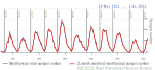
\includegraphics[width=0.8\linewidth]{Figs/sunspots.pdf}
    \caption{Ciclos solares en los últimos 100 años observados a partir del número de manchas solares. Fuente WDC-SILSO, Royal Observatory of Belgium, Brussels}
    \label{fig:100ysn}
\end{figure}

\section{Propagación de CR a través del Campo Geomagnético}

La Tierra está rodeada por un campo magnético casi dipolar generado por las corrientes eléctricas de su núcleo. A esta región del espacio donde el campo magnético terrestre es predominante sobre el campo magnético interplanetario se llama magnetosfera y tiene una forma asimétrica, como se muestra en la figura \ref{magnetosfera}. 

El viento solar interactúa con el campo magnético comprimiéndolo en la dirección del Sol y lo estira en la dirección opuesta, creando una cola magnética (figura \ref{magnetosfera}).  De la misma forma, la interacción de los RC primarios con el campo geomagnético terrestre también modula su intensidad a nivel del suelo. El campo geomagnético desvía las trayectorias de las partículas primarias según su rigidez $R$, que es la relación entre su cantidad de movimiento $p$ y su carga $q$. 
\begin{equation}
    R=\frac{p}{q}=r_{L}B.
\end{equation}
Donde $r_L$ representa el radio de Larmor, parámetro usado para determinar la capacidad que tiene una partícula de penetrar el campo magnético en una ubicación específica. En un campo geomagnético dipolar como el de la Tierra, el momento mínimo por carga que una partícula debe tener en una ubicación determinada se puede describir con la rigidez de corte $R_C$:
\begin{equation}
    R_C=\kappa\frac{1}{L^{\alpha}}
    = \frac{M cos^{4}\lambda}{4r^{2}},
\end{equation}
donde $L$ es el parámetro McIlwain, que denota la distancia a la que una línea de campo magnético cruza el plano ecuatorial, $M$ representa el momento dipolar, $r$ la distancia desde el centro del dipolo (en unidades de radios terrestres), $\lambda$ la latitud geográfica, y las constantes $\kappa$ y $\alpha$ valen $\approx 14.823GV$ y  $2,0311$ respectivamente. Esta ecuación es válida solo para latitudes altas e ignora la geometría del campo. Además, la estructura del campo magnético de la Tierra es mucho más intrincada que la de un dipolo simple. Por tanto, para calcular RC en cualquier campo magnético se deben realizar cálculos numéricos.

\begin{figure}
    \centering
    \includegraphics[width=0.7\linewidth]{Figs/Schematic-representation-of-the-near-Earths-magnetosphere.png}
    \caption{Representación esquemática del campo geomagnético terrestre. Fuente \cite{tenerani_2012}}
    \label{magnetosfera}
\end{figure}
%%%% ESTO VA ABAJOOOOOOOOOOOOOOO
\textbf{Decrecimientos Forbush (FD)}: Son disminuciones breves de la intensidad de los GCR seguidas de una lenta recuperación, que suele durar varios días (\cite{forbush_1954}). Inicialmente se atribuyeron a las erupciones solares, pero más tarde se descubrió que estaban causados por CME (\cite{lingri_2016}). Este fenómeno corresponde a los eventos de rayos cósmicos más importantes registrados en los monitores de neutrones terrestres y tienen características diferentes en relación con los parámetros de actividad solar durante las distintas fases de los ciclos solares. La amplitud de las disminuciones de intensidad de los rayos cósmicos que miden estos monitores varía con la diferente rigidez de corte de cada estación alcanzando registros de hasta un $25\%$ (\cite{cane2000}).

 Los FD pueden clasificarse en dos tipos: no recurrentes y recurrentes. Los no recurrentes tienen un inicio repentino y están asociadas a perturbaciones transitorias del viento solar. Tienen perfiles asimétricos y se ven afectados por el área, la velocidad y la fuerza del campo magnético irregular de las CME (\cite{cane2000}, \cite{lingri_2016}). Contrariamente los decrecimientos recurrentes tienen un inicio gradual, un perfil simétrico y están bien asociadas con corrientes de viento solar de alta velocidad corrotantes que son más frecuentes en los periodos de alta actividad solar (\cite{lingri_2016}, \cite{kallaya_2021},\cite{wang_2023}). La figura \ref{forbush}  muestra un FD registrado en mayo de 2005 por el observatorio Pierre Auger y el monitor de neutrones de Los Cerrillos (Chile). 
\begin{figure}[H]
    \centering
    \includegraphics[width=0.6\linewidth]{Figs/mauro_forbush.png}
    \caption{Perfil de un Decrecimiento Forbush ocurrido el 13 de mayo del 2005. Se observa la comparación del evento medido por el Observatorio Pierre Auger en contraste a la señal obtenida con el monitor de neutrones de Los Cerritos en Chile, escogido por la similitud de las rigideces de corte geomagnético. Fuente \cite{asorey_2012}}
    \label{forbush}
\end{figure}
En el caso de los FD no recurrentes, la disminución del flujo de rayos cósmicos se debe al efecto de apantallamiento que produce la estructura magnética de la ICME y la onda de choque que la acompaña, tal como se representa en la figura \ref{icme} (\cite{papaioannou_2020}). El campo magnético de la ICME es más intenso y turbulento que el del viento solar, lo que dispezrsa más a los rayos cósmicos y los desvía de su trayectoria original (\cite{belov_2009}). Además, la onda de choque de la ICME comprime el plasma y el campo magnético, lo que crea una barrera que dificulta el paso de los rayos cósmicos. Estos efectos son más notorios para las partículas de menor energía, que son más sensibles a la fuerza de Lorentz que ejerce el campo magnético. Así, los rayos cósmicos que atraviesan una ICME sufren una modulación de su flujo, su espectro de energía y su anisotropía.

\section{Propagación de CR a través de la atmósfera terrestre}

Cuando los CR primarios llegan a la atmósfera terrestre, chocan con los átomos del aire y producen una lluvia de partículas EAS que tienen menos energía que el primario. Algunas de estas partículas pueden decaer o interactuar nuevamente, generando una reacción en cadena (\cite{gaisser1990}) que se detiene cuando la energía del primario se disipa o se alcanza el nivel del suelo.

Durante el desarrollo de una EAS las partículas recorren una cierta cantidad de materia a medida que atraviesan la atmósfera. Este parámetro comúnmente llamado profundidad atmosférica $X(h)$, depende de la altura $h$ sobre el nivel del mar y de la densidad del aire $\rho(h)$.  
\begin{equation}
X_{v}= \int_{h}^{\infty} \rho (h') dh'.
\label{eq:eq2}
\end{equation}
Las interacciones producidas a lo largo del desarrollo de la cascada a través de una cierta cantidad de materia $X(h)$ permiten identificar tres componentes principales: una electromagnética, que está conformada por electrones, positrones y fotones; otra hadrónica, constituida de piones, kaones y bariones, y una componente muónica, generada por el decaimiento de piones y kaones cargados. La figura \ref{fig:fig3} ilustra los procesos de interacción mostrados anteriormente y cómo éstos generan cada una de las componentes. Como se observa en la imagen, la producción de partículas secundarias está mediada por interacciones electromagnéticas y hadrónicas que describiremos con un poco más de detalle a continuación.

\begin{figure}[htb!]
\centering
    \begin{center}
        \includegraphics[width=0.5\textwidth]{Figs/componentes_cas.jpg}
    \end{center}{}
    \caption[Esquema del desarrollo de una EAS iniciada por un hadrón.]{Esquema del desarrollo más probable de una EAS iniciada por un hadrón \cite{mauro:tesis}. En la figura se observa el decaimiento del hadrón en piones cargados y neutros, y estos a su vez, al decaer, generan fotones, electrones y muones. Se identifican tres componentes: electromagnética, muónica y hadrónica.}
    \label{fig:fig3}
\end{figure}

\subsection{Interacciones electromagnéticas}
Están presentes cuando el primario incidente es un fotón o un electrón. Estas partículas pueden crear o emitir otras partículas del mismo tipo al interactuar con los átomos del aire. Por ejemplo, los fotones pueden crear pares de electrones y positrones, y estos pueden emitir más fotones al frenarse (bremsstranhlung). Este proceso se detiene cuando los fotones tienen una energía de $1.02 MeV$. En el caso de un núcleo de aire con carga $Z$ y número atómico $A$, los procesos de producción son (\cite{heitler}):
 %para quienes el principal canales de interacción son la producción de pares y radiación de frenado. E
\begin{equation}
\begin{split}
&Bremsstrahlung\quad e \quad \xrightarrow{Y^{A}_{Z}} \quad e\gamma ,  \quad y \\
&Pares \quad \gamma \xrightarrow{Y^{A}_{Z}} \quad e^{+}e^{-}. \\
\end{split}
\end{equation} 
Otros procesos electromagnéticos que influyen en esta pérdida de energía y deben ser considerados son:

\textbf{La pérdida de energía por Ionización} de una partícula cargada que atraviesa la materia con un espesor $\lambda$ que es descrita por la ecuación de Bethe-Bloch:
\begin{equation}
dE_{i} = \frac{\lambda \gamma^{2}z^{2}}{\gamma^{2}-1}\kappa_{1}(ln(\gamma^{2}-1)- \beta^{2}+\kappa_{2}).
\label{eq:eq20}
\end{equation}

Donde $\beta = v/c $ es la velocidad de la partícula en unidades de la velocidad de la luz, $\gamma$ es el factor de Lorentz, $z$ es la carga de la partícula ionizada en unidades de $e$. Las dos constantes $\kappa_{1}= 0.153287$ $ MeV g^{-1}$ y $\kappa_{2}= 9.386417 $ $MeV g^{-1}$ son los valores correspondientes para el aire (\cite{Heck1998}). Esta expresión es usada para calcular la perdida por energía de ionización a través de la trayectoria de la partícula. Por ejemplo, la pérdida de energía de muones como función de su energía está representada en la figura \ref{fig:fig4}.
\begin{figure}[htb!]
\centering
        \includegraphics[width=0.7\textwidth]{Figs/Bethe_Muons.png}
        \caption[Ecuación de Bethe-Bloch para los muones.]{Pérdida de energía de Muones en el aire como función del factor de Lorentz . Están indicadas las contribuciones de la ionización (línea seccionada) y la producción de pares (línea punteada). Fuente: \cite{Heck1998}}
        \label{fig:fig4}
\end{figure}

La \textbf{Dispersión múltiple de Coulomb} que ocurre cuando las partículas cargadas son dispersadas por el campo eléctrico Coulombiano de los núcleos de aire. Allí la dirección de propagación es alterada pero no cambia la energía de la partícula. La distribución angular de esta dispersión es descrita por la teoría de Moliére (\cite{Heck1998}).  

\subsection{Interacciones hadrónicas}
%%%%% NEW
Las interacciones hadrónicas son un componente fundamental en el estudio de las EAS. Aunque la cromodinámica cuántica proporciona una base sólida para entender las interacciones fuertes, los procesos con múltiples partículas producidas en las interacciones hadrónicas aún no pueden ser calculados con precisión. Para superar esta limitación, se han desarrollado modelos que hacen suposiciones adicionales y utilizan parametrizaciones fenomenológicas y empíricas (\cite{Allen}). Estos modelos son esenciales para interpretar las EAS y deben estar optimizados para un amplio rango de energías. Además, es crucial que se actualicen constantemente a medida que se obtienen más datos de los aceleradores o de grandes instrumentos como el Observatorio Pierre Auger \cite{andrada_2021}. Las interacciones hadrónicas generan piones cargados y neutros ($\pi^{-},\pi^{+},\pi^{0}$), así como kaones, que tienen una tendencia mayor a decaer que a interactuar. Los canales de decaimiento más probables para estas partículas son los siguientes:
\begin{align*}
\pi^{0} &\rightarrow \gamma\gamma \quad [{98.823 \pm 0.034}{\%}], \\
\pi^{0} &\rightarrow e^{+}e^{-} \gamma \quad [{1.174 \pm 0.035}{\%}], \\
\pi^{+} &\rightarrow \mu^{+}\nu_{\mu} \quad [{99.98 \pm 0.00004}{\%}], \\
\pi^{-} &\rightarrow \mu^{-}\nu_{\mu} \quad [{99.98 \pm 0.00004}{\%}], \\
K^{+} &\rightarrow \mu^{+}\nu_{\mu} \quad [{63.56 \pm 0.11}{\%}], \\
K^{+} &\rightarrow \pi^{0}e^{+}\nu_{e} \quad [{5.07 \pm 0.004}{\%}], \\
K^{+} &\rightarrow \pi^{+}\pi^{0} \quad [{20.67 \pm 0.08}{\%}] \quad y \\
K^{+} &\rightarrow \pi^{+}\pi^{+}\pi^{-} \quad [{5.583 \pm 0.024}{\%}].
\end{align*}
Estos procesos contribuyen a la componente electromagnética y muónica de las EAS. Más específicamente, la componente muónica en las EAS es de particular interés debido a las propiedades relativistas de los muones y su larga vida media. Esta componente ofrece una visión directa de las primeras interacciones hadrónicas y las propiedades del hadrón inicial. Los muones de alta energía desencadenan sub-cascadas electromagnéticas y hadrónicas en la lluvia a través de interacciones tipo:
\begin{align}
\mu^{\pm} \quad &\xrightarrow{Y^{A}_{Z}} \quad \mu^{\pm}e^{+}e^{-}, \\
\mu^{\pm} \quad &\xrightarrow{Y^{A}_{Z}} \quad \mu^{\pm} + \text{hadrones}.
\end{align}  
%%%%%%%%%%%%%%%%%%%%%%%%%%%%%%%%%%%%%%%%%%%%%%%%%%%%%%%%%
%%%%%%%%%%%%%%%%%%%%%%%%%%%%----->SECCIÓN 3<-----%%%%%%%%%%%%%%%%%%%%%%%%%
\newpage
\newpage

\chapter{El Observatorio Pierre Auger}

El Observatorio Pierre Auger es el observatorio de rayos cósmicos más grande del mundo, con un área de detección de alrededor de  $3000 km^{2}$ enfocado en la detección indirecta de rayos cósmicos de ultra alta energía $(E > 10^{18} eV)$, cuya tasa de arribo a la tierra está entre 1 partícula $ km^{2}/year$ a 1 partícula $km^{2}/century$. El observatorio es un arreglo híbrido, que está constituido principalmente por dos tipos de detectores: los telescopios de fluorescencia atmosférica FD y los detectores Chérenkov de superficie SD. El objetivo de este detector híbrido es proporcionar estadísticas de alto nivel y reducir las incertidumbres sistemáticas en la medición de las energías de los rayos cósmicos. A continuación, se hará una revisión de las generalidades de cada uno de estos detectores.    

\section{Detector de Fluorescencia}
El detector de fluorescencia está diseñado para detectar el desarrollo longitudinal de las lluvias de partículas secundarias generadas por rayos cósmicos de muy alta energía. Esto es posible gracias a que al propagarse por la atmósfera los RC secundarios excitan el nitrógeno liberando luz fluorescente en el rango de 300nm a 430nm. El criterio principal de su diseño es la detección de cada lluvia con energías de al menos $10^{19}eV$ (\cite{Aab_2015}). Este arreglo consta de 24 telescopios independientes distribuidos en 4 sitios, cada uno con un campo de visión de $30^o x 30^o$ . En este fenómeno, el número de fotones producidos es proporcional a la energía de la componente electromagnética de la lluvia y al número total de partículas generadas a cierta profundidad atmosférica (\cite{asorey}). \footnote{La profundidad atmosférica $X$, es un parámetro que permite estimar la cantidad de materia con la que ha interactuado el primario al penetrar en la atmósfera. La expresión:
\begin{equation}
X_{v}= \int_{h}^{\infty} \rho (h') dh',
\label{integral}
\end{equation}
}

\begin{figure}[!ht]
\centering
\includegraphics[width=1\textwidth]{Figs/FD_auger_composition.png}
\caption{a) Mapa donde se muestra la ubicación del Observatorio Pierre Auger y de sus sistemas detectores. Los puntos amarillos corresponden a los detectores de superficie SD, y los 4 puntos negros en las fronteras, corresponden a la ubicación de los detectores de fluorescencia FD (\cite{asorey}). b) Los puntos grises muestran las posiciones de las estaciones de detectores de superficie. Los semicírculos en gris claro indican los campos de visión de 24 telescopios de fluorescencia situados en cuatro edificios en el perímetro de los detectores de superficie (\cite{FD_auger}). c) Esquema de uno de los cuatro edificios con seis telescopios de fluorescencia en su interior logrando un campo de visión de $180^{o}$ (\cite{FD_auger}). d) Estructura de un telescopio FD. El sistema de apertura consta de un diafragma, un anillo corrector y un filtro UV. Los demás componentes ópticos son el Los otros componentes ópticos son el espejo y la cámara, que incluye un conjunto de 20x22 PMT (\cite{dedonato_2007}).}
\label{fd_auger}
\end{figure}

El arreglo utiliza un filtro UV para dejar pasar solo luz ultravioleta (UV) en el rango de 330 a 380 nanómetros que corresponde al rango de interés para las observaciones. Además, los telescopios están diseñados para funcionar únicamente durante noches despejadas sin Luna, lo que reduce el ruido de fondo y mejora la precisión de las mediciones. 

\section{Detector de superficie SD}

El Observatorio Pierre Auger cuenta con un detector de superficie que comprende una matriz de 1660 estaciones de detección de agua Cherenkov (WCD), abarcando un área total de 3000$km^{2}$. Estas estaciones están distribuidas en una red hexagonal de $1.5km$ entre cada una. Dicha configuración está diseñada para estudiar el desarrollo transversal de todas las lluvias de partículas generadas por partículas primarias de al menos $10^{18} eV$ a nivel del suelo.

Dado el tamaño del área cubierta, las estaciones deben operar de manera autónoma y requerir poco mantenimiento (\cite{SD_auger}). Por lo tanto, estos detectores están interconectados a través de una red inalámbrica de área local (WLAN), cuyo receptor principal es el telescopio de fluorescencia (FD) más cercano, que se encarga de transmitir los datos a la central de recopilación principal CDAS.

\subsection{Efecto Chérenkov}

Cuando una partícula con carga se mueve a través de un medio, su pérdida de energía aumentará a medida que la densidad del medio se incremente. Si consideramos que la densidad $\rho$ del medio es constante y que \textit{b} es el parámetro de impacto, la energía que pierde la partícula al atravesar una sección de longitud \textit{dl} dentro de un cilindro de radio \textit{a}, cuyo eje coincide con la dirección de movimiento, se puede expresar como $\frac{dE}{dl} = \rho \frac{dE}{dX}$. Esta pérdida de energía está determinada por el flujo del vector de Poynting, con la componente longitudinal $E_{1}$ del campo eléctrico, y con la componente transversal del campo magnético $B_{3}$ presentes en el medio, en función de la frecuencia $\omega$ (\cite{fermi_1940}).
\begin{equation}
    \frac{dE}{dl} = -ca \mathcal{R}\left(\int_{0}^{\infty} B^{*}E_{1}(\omega) \, d\omega\right)
    \label{fermi1}
\end{equation}
%%%%%%%%%%%%%%%%% PARENTESISSSSS
Consideremos una partícula cargada que se desplaza a una velocidad $v=\beta c$ a través de un medio con una constante dieléctrica $\epsilon(\omega)$ y un número atómico $Z$. En este escenario, la longitud de onda de la radiación emitida se modificará debido a la presencia del medio de la siguiente manera:
\begin{equation}
\lambda^{2}=\frac{\omega^{2}}{v^{2}}(1-\beta^{2}\epsilon(\omega))
\label{lamdamod}
\end{equation}
Teniendo en cuenta las expresiones para los campos $E$ y $B$, el integrando de la ecuación \ref{fermi1} obtenemos:
\begin{equation}
B^{}E_{1}(\omega)=\left(\frac{Ze}{c}\right)^2 \left(-i\sqrt{\frac{\lambda^{}}{\lambda}}\right)\left(1-\frac{1}{\beta^{2}\epsilon(\omega)}\right)exp[-a(\lambda+\lambda^{*})]\omega
\end{equation}
En este caso, si $\lambda$ es un número imaginario puro, $\lambda^{*}=-\lambda$ lo que haría 
$exp[-a(\lambda+\lambda^{*})] = 1$ y por consiguiente la expresión \ref{fermi1} sería independiente de $a$, donde parte de la energía escapa al infinito en forma de emisión coherente de radiación (\cite{asorey}). Esto sucede si $\epsilon$ es real, es decir que el medio no es absorbente y que $\beta^{2}\epsilon(\omega)>1$ ó $\beta=\frac{1}{\sqrt{\epsilon(\omega)}}$, o en otras palabras, si la velocidad de la partícula cargada es mayor que la velocidad de la luz en el medio a una frecuencia $\omega$, fenómeno conocido como \textit{Efecto Cherenkov}.

Si el medio es ligeramente absorbente la expresión \ref{fermi1} queda como:
\begin{equation}
\left(\frac{dE}{dl}\right)_{Cherenkov}=\left(\frac{Ze}{c}\right)\int{\beta^{2}\epsilon(\omega)>1} \omega\left(1-\frac{1}{\beta^{2}\epsilon(\omega)}\right)d\omega
\end{equation}
donde se observa que la emisión de radiación depende de la frecuencia. En el caso del agua, en el espectro visible, la radiación Cherenkov se produce a longitudes de onda cortas, donde  $n(\omega) \approx \sqrt{\epsilon(\omega)}$ aumenta levemente con la frecuencia. El ángulo de emisión de la radiación está definido entonces por:
\begin{equation}
cos\theta_{c}=\frac{1}{\beta\sqrt{\epsilon(\omega)}},
\end{equation}
Para el rango de frecuencias de interés (cerca del ultravioleta), el valor del índice de refracción puede ser considerado constante, con lo que podemos obtener el número de fotones Cherenkov producidos en un intervalo de longitudes de onda como sigue,
\begin{equation}
N=2\pi \alpha_{EM}l\left(1-\frac{1}{\beta^{2}n^{2}}\right)\left(\frac{1}{\lambda_{2}}-\frac{1}{\lambda_{1}}\right),
\label{cherenkovnumber}
\end{equation}


%%%%%%%%%%%%%%%%% PARENTESISSSSS

%EN ALGÚN MOMENTO DE LA VIDA \hbar cambió por \hslash en esta joda y no me enteré....

Donde $\alpha_{EM}=(e^2/ \hslash c)$ es la constante de estructura fina. Además, el momento de una partícula con masa en reposo $m_{0}$ y velocidad $\beta c$ es $p\equiv mv = \beta \gamma m_{0}c$, lo que permite calcular el número de fotones emitidos por una partícula con momento $p$ al recorrer una longitud $l$ en un medio con índice de refracción $n$. En el caso de los tubos fotomultiplicadores utilizados en el Observatorio Pierre Auger, que son sensibles al rango de $300 - 570nm$, es posible definir dos propiedades clave en la respuesta posterior de los detectores Cherenkov:
\begin{itemize}
\item La radiación solo se emite cuando $\beta>1/n$.
\item El número de fotones emitidos por unidad de longitud tiende a un valor constante (ver figura \ref{stopping_cherenkov}), que solo depende del rango de longitudes de onda considerado, del índice de refracción del medio y la distancia recorrida en dicho medio. De esta manera, la señal en el detector no proviene de la energía depositada, sino de la cantidad de fotones producidos, es decir, de la distancia recorrida por la partícula en el agua (\cite{asorey}).
\end{itemize}
\begin{figure}
\centering
\includegraphics[width=1\textwidth]{Figs/cherenkov_stopping.png}
\caption{a) Arriba: ilustración de la polarización del medio inducida por el paso de una partícula relativista. Abajo: Construcción del frente de onda de Cherenkov. Fuente: \cite{deNaurois:2015oda} b) Esquema Producción de fotones Cherenkov en la banda $300 nm < \lambda < 570 nm$ según la ecuación \ref{cherenkovnumber} como función del impulso. La línea punteada corresponde a un electrón y la sólida a un muón luego de haber recorrido 1 cm en agua líquida. Se puede observar que la cantidad de fotones tiende rápidamente a un valor constante de $\thicksim 315$ fotones por centímetro incluyendo el momento más probable para las dos partículas. Fuente \cite{asorey}}
\label{stopping_cherenkov}
\end{figure}
\subsection{El detector Cherenkov}
 
%Para ampliar las capacidades del observatorio a energías más bajas, también se despliega una región de relleno de estaciones SD con un espaciado de 750 m (SD-750) [68]. 
Cada Estación de Detección (SD) se compone de un recipiente cilíndrico con una superficie de base de 10$m^{2}$, lleno con 12 $m^{3}$ de agua de alta pureza que permite una mínima absorción de luz ultravioleta cercana. Esta agua se encuentra dentro de una bolsa fabricada con Tyvek, un material reflectante. Cuando las partículas relativistas atraviesan el volumen de agua, generan radiación Cherenkov que es reflejada y dispersada por el Tyvek en el interior del recipiente, lo que incrementa la probabilidad de detección (\cite{SD_auger}).

Esta radiación es captada por tres tubos fotomultiplicadores (en adelante PMT, por sus siglas en inglés) Photonis XP1805/D1 de 9 pulgadas de diámetro (\cite{Aab_2015}), dispuestos de forma simétrica en la parte superior del tanque. Las señales analógicas de los PMT son convertidas a formato digital en la electrónica de la estación mediante convertidores de tipo flash de analógico a digital (FADC). Cada PMT registra el pulso que genera la detección de fotoelectrones que se caracteriza por tener un crecimiento rápido y un posterior decaimiento exponencial como se muestra en la figura \ref{fig:PMT}.

%Cada SD consta de un tanque cilíndrico de 10$m^{2}$ de base con 12 $m^{3}$ de agua ultra pura que permita una baja absorción del ultravioleta cercano, dentro de una bolsa con un material reflectante realizada en Tyvek. La radiación Cherenkov producida por el paso de partículas relativistas a través del volumen de agua, es reflejada y difundida por el Tyvek en el interior, maximizando la probabilidad de detección \cite{asorey} y es registrada con tres tubos fotomultiplicadores (PMT) Photonis XP1805/D1 de 9 pulgadas de diámetro, (\cite{Aab_2015}) colocados simétricamente en la parte superior del tanque. Las señales analógicas provenientes de los PMT son digitalizadas en la electrónica de las estación mediante conversores analógicos digitales tipo flash (FADC).
\begin{figure}[!ht]
  \centering
\includegraphics[width=1\textwidth]{Figs/SD_componentes.png}
  \caption{Estructura de un detector de superficie SD. A la izquierda se observa el exterior de un detector WCD del Observatorio ubicado en la Pampa Amarilla. A la derecha vemos una representación de su interior: Al entrar la partícula cargada al agua se produce un cono de luz Cherenkov, estos fotones son reflejados por las paredes del detector y recogidos por los PMT ubicados simétricamente en la superficie superior. \cite{SD_auger}}
  \label{fig:SD_auger}
\end{figure}



\begin{figure}[h!]
  \centering
\includegraphics[width=0.6\textwidth]{Figs/PMTs_signal.png}
  \caption{Señal del ánodo de cada PMT. Estas señales son digitalizadas mediante seis conversores FADC de 10 bits a una velocidad de muestreo de 40 MHz. La traza consiste en un bloque contiguo de 768 bines de señal de 25 ns cada uno, totalizando $19.2 \mu s$. Fuente: (\cite{asorey})}
  \label{fig:PMT}
\end{figure}
Una de las ventajas de usar detectores Cherenkov es que se puede diferenciar el paso de los muones (o su decaimiento) y la absorción de los electrones. Los muones atmosféricos (con energías típicas de $E_\mu \thicksim 3GeV$), depositan en el detector solo una pequeña fracción de su energía cinética de tal forma que son capaces de atravesarlo. (El poder de frenado de muones en agua es de $\thicksim 2 MeV cm^{-1}$ en un amplio rango de energías ) (\cite{asorey}). La señal Cherenkov producida por muones depende únicamente de la longitud recorrida en el agua, determinada por la geometría del detector y la dirección del muón. Para muones con $E_\mu < 390 MeV$, su rango es menor que la profundidad del detector en posición vertical. Estos muones depositan toda su energía en el detector y pueden decaer en su interior.

Por el contrario, los electrones cuyo rango de energía típico es de $\thicksim 20MeV$, poseen un poder de frenado de $\thicksim 2MeV cm^{-1}$, lo que provoca que al ingresar al agua se produzca una absorción total en el volumen del detector. El número total de fotones producidos, y por ende la señal registrada, muestra una fuerte dependencia de la energía inicial del electrón, alcanzando un máximo para trayectorias verticales que atraviesan completamente el detector ($\thicksim 3.8 x 10^{4}$ fotones). De esta forma, el detector actúa como calorímetro de electrones absorbiendo toda su energía cinética, la señal que se registra está relacionada solo con la emisión de fotones Cherenkov que se detiene antes de absorber completamente al electrón. 

La diferenciación entre las señales producidas por fotones y muones se evidencia en la figura \ref{cargahist} donde contrasta la carga depositada durante un tiempo y medida por un tubo fotomultiplicador del observatorio. El pico inicial refleja la distribución de señales principalmente generadas por la componente electromagnética, sumada al efecto del umbral de detección. El segundo pico, por su parte, se relaciona con el paso de muones que atraviesan verticalmente el detector. La posición del pico para un muón central y vertical medido por un PMT del Observatorio es de $(1.03\pm0.02)$ \cite{asorey}.

\begin{figure}[h!]
  \centering
\includegraphics[width=0.6\textwidth]{Figs/histograma_carga.png}
  \caption{carga depositada durante un tiempo y medida por un tubo fotomultiplicador del observatorio. El pico inicial refleja la distribución de señales principalmente generadas por la componente electromagnética, sumada al efecto del umbral de detección. El segundo pico, por su parte, se relaciona con el paso de muones que atraviesan verticalmente el detector. Fuente: (\cite{asorey})}
  \label{cargahist}
\end{figure}
Algunos parámetros de importancia referentes a los detectores cherenkov del Observatorio que serán necesarios para las secciones siguientes son:
\begin{itemize}
    \item \textbf{Cuentas ADC de pico:} Es la magnitud correspondiente al valor de salida del conversor FADC de tal forma que $1ADC_{p}= 1.95mV$ 
    \item \textbf{Bin de la señal:} Intervalo entre dos pulsos sucesivos. Considerando que el conversor tiene una tasa de muestreo de 40MHz, se establece que $1bin\equiv \frac{1}{40MHz} = 25ns$
    \item \textbf{Cuenas ADC de carga:} Unidad luego de integrar temporalmente la señal en $ADC_{p}$, restando la línea base.
    \item \textbf{$VEM$ (\textit{Vertical Equivalent Muon}):} Es la carga total depositada por un muón que atraviesa completamente a un SD de forma vertical, un $MCV$ (\textit{muón central y vertical}). $1VEM=\frac{q_{VEM}}{1.03}ADC_{q}=240MeV$.
    \item \textbf{$VEM_{p}$:} Es el equivalente a la altura máxima del pulso típico de la señal producido por un $MCV$: $1VEM_{P}=\frac{I_{VEM}}{1.03}ADC_{p}=240MeV$.
    \item \textbf{Relación carga sobre pico $AoP$: } Es posible tener una idea de la respuesta impulsional del detector frente a los muones, relacionando las cargas integradas $(ADC_{q})$ y los voltajes $(ADC_{p})$ en la zona de pico de muones del histograma. De tal forma que: $AoP=\frac{ADC_{q}}{ADC_{p}}$ que correspondería a un parámetro fundamental de calibración.
    \item \textbf{Sistema de disparo (trigger):} Es la estructura de 5 niveles que se establecen sobre el nivel de detección para seleccionar las señales producidas por los rayos cósmicos de interés sobre el fondo, con el objetivo de descartar ruidos y eventos físicos no relevantes para el observatorio. Por lo anterior, cada uno de los detectores registra de forma diaria un promedio de tres eventos diarios por detector.
\end{itemize}

\section{Medición del fondo de rayos cósmicos}

El fondo de rayos cósmicos secundarios en la superficie de la Tierra es el resultado de las interacciones de los rayos cósmicos galácticos (GCRs) y el viento solar con la atmósfera terrestre. Como se describió en el capítulo 1, en el espectro de energía predominan estas dos fuentes (ver \ref{fig:spectrum}). Podría decirse que este fondo corresponde a un flujo constante de partículas que varía levemente debido a la actividad solar periódica y transitoria. El Observatorio Pierre Auger, aunque está optimizado para la identificación de partículas de ultra alta energía, tiene dos modos de detección alternativos de baja energía que registran el flujo de partículas secundarias al nivel de los detectores de superficie (SD): El modo Scaler y el modo Histograma. Este trabajo de investigación explora las características y propiedades del modo scaler aplicado al estudio del fondo de radiación natural y su variabilidad estrechamente relacionada con la actividad solar, aprovechando la capacidad de recolección de datos, la cantidad de detectores y la superficie cubierta por este arreglo. A continuación, veamos en qué consisten estos dos modos de baja energía.

\subsection{Modo Scaler}

En 1997, se propuso la implementación en el observatorio de un modo de detección que estuviera destinado a caracterizar el fondo y  con este, identificar lluvias atmosféricas extendidas originadas por los fotones provenientes de GRBs (destellos de rayos gamma)(\cite{asorey} \cite{bertou_2011}). Los GRB consisten en una emisión súbita de rayos gamma en periodos cortos de tiempo ($\cdot 10^{-3}s - \cdot 10^{2}s$) que continúa en la emisión de fotones cada vez menos energéticos (rayos X hasta radio). El espectro en energía de los fotones gamma observados durante la ocurrencia de un GRB, muestran que podrían llegar hasta energías de varios GeV (\cite{Bernlöhr_1996}).

%El espectro de energía de los fotones gamma que han sido observados y reportados pueden llegar a energías en el rango de unidades de $GeV$ 

El modo scaler consiste en determinar las tasas de conteo de pulsos individuales de cada SD en escalas de tiempo de un segundo \cite{asorey}. Con este método, se puede determinar el flujo de fondo sobre el arreglo y a partir de éste, identificar excesos generados por fenómenos transitorios diversos como por ejemplo un GRB, también pueden dar una idea de la tasa de rayos cósmicos de baja energía influidos por la modulación solar.

Como es de esperarse, no todas las señales registradas con el SD corresponden a datos válidos para la determinación de este flujo. En primer lugar, la diferencia entre la línea base y el voltaje del pico del pulso debe cumplir las siguientes condiciones:

\begin{itemize}
    \item Del 20 de Marzo hasta el 20 de Septiembre de 2005, este voltaje debe ser mayor a 3ADC
    \item Desde el 21 de Septiembre del 2005, la diferencia de voltajes debe comprender entre: $3ADC < (V_{p}-V_{b}) \leq 20ADC $
\end{itemize}

Esta diferencia de periodos se sustenta en la necesidad de implementar un umbral de detección superior que permita una mejor relación señal a ruido \cite{GAP_2005}, y así superar las limitaciones en los datos que se venían recolectando. Dichos cambios en los umbrales fueron implementados desde el 21 de Septiembre del 2005.

Los pulsos recopilados son guardados enviados una vez por segundo para su almacenamiento. Cada segundo de datos contiene: el tiempo en que se realizó el registro, número de estaciones activas, el número total de pulsos contados en todo el arreglo, y los conteos de pulsos para cada SD. Finalmente se obtiene un archivo de datos por día. Luego de esto, se deben eliminar los detectores que muestren inestabilidades respecto a la media, ruido producido por rayos, inestabilidades térmicas y relámpagos originados en tormentas eléctricas.  la tasa de recuento es de unos 2 kHz por detector y la energía depositada es de unos 15 a 100 MeV [74]. Usando simulaciones, se determina que las partículas primarias que crean las partículas secundarias contadas por el Scaler están entre 10 GeV y unos 10 TeV con una mediana de 90 GeV [76]
%%%% CITAR ESTE PÁRRAFO ES TOMADO DE MARTIN

\subsection{Modo histograma}

El modo Histograma permite estudiar la variación de la tasa de conteo en diferentes rangos de energía depositada, asociados con diversas energías primarias de rayos cósmicos galácticos (GCRs). En el sistema de detección del Observatorio, corresponde al registro de los pulsos del fondo de radiación en intervalos de tiempo de 61 segundos \cite{asorey} . Estos registros permiten realizar la calibración del detector en un intervalo de tiempo determinado respecto a su respuesta impulsional y acompañan los eventos filtrados y almanecados por el sistema de trigger principal. 

%Se construyen en cada detector a partir de los histogramas de pico o pulsos y también de la carca depositada por cada señal. 

Después del proceso de calibración, a partir del VEM se pueden construir histogramas de energía depositada de hasta aproximadamente 1 GeV. El modo Histograma permite estudiar la variación de la tasa de conteo en diferentes rangos de energía depositada, asociados con diversas energías primarias de rayos cósmicos galácticos (GCRs) (\cite{asorey}, \cite{masias_2017}). Los dos rangos de energía de mayor interés son: el rango asociado a las energías depositadas en el modo Scaler (energía entre 60 MeV y 120 MeV), y el relacionado con las energías depositadas por muones con incidencia vertical (energía entre 200 MeV y 280 MeV), también denominado "banda muónica". 

Los modos scaler e histograma están fuertemente relacionados puesto que la integral del histograma de carga, por construcción, representa el número de señales registradas en ese minuto. Ajustando adecuadamente los límites de esta integración, teóricamente debería ser posible recuperar las tasas de los Scalers de ese detector.  

%%%%%%%%%%%%%%%%%%%%%%%%%%%%----->SECCIÓN 3<-----%%%%%%%%%%%%%%%%%%%%%%%%%
\newpage
\chapter{Modulación del fondo de Rayos Cósmicos debido a la actividad Solar}

%%%%%%%%%%%%%%%%%%%%%%%%%%%%% NEWW
En este último capítulo, presentaremos los resultados obtenidos del estudio de la modulación de los GCR debido a la actividad solar, sobre los datos de scaler del observatorio Pierre Auger. Como se describió en el capítulo 1, la interacción entre los GCR y el viento solar provoca cambios en el flujo de fondo al nivel del suelo.  Los estudios previos realizados en el Observatorio han demostrado que el modo scaler es altamente sensible a las condiciones del medio interplanetario determinadas por la actividad solar (\cite{Martin_Schimassek2022}). Esta sensibilidad permite que los datos recopilados en este modo scaler proporcionen información complementaria a la obtenida a través de los monitores de neutrones, abriendo una ventana energética de observación diferente para los rayos cósmicos de baja energía.
%El viento solar, que se ve afectado por fenómenos periódicos como la rotación solar de \~27 días, el ciclo de 11 años que está asociado a emisiones de plasma desde la corona y a un cambio en la frecuencia de las eyecciones de masa coronal (CME) (\cite{belov_2021} entre otros).

Comenzaremos con una descripción de los datos y las fuentes que hemos utilizado para este estudio, seguido de una explicación de cómo se procesaron los datos en modo scaler del arreglo de detectores para garantizar la fiabilidad. A continuación, realizaremos una comparación entre las mediciones realizadas por detectores de neutrones (NM) y las obtenidas en el Observatorio Pierre Auger, destacando las ventajas y desventajas de cada uno en el contexto de nuestro estudio. Finalmente, discutiremos los efectos de la actividad solar en el fondo de rayos cósmicos a corto y largo plazo, proporcionando una visión completa de cómo la actividad solar puede influir en la detección de GCR.

\section{Datos}

En este trabajo, se utilizaron las siguientes bases de datos :
\begin{enumerate}

\item scalers del Observatorio Pierre Auger: Los datos son corregidos por presión y temperatura usando el software \textit{scalerAnalysis} cuya metodología describiremos en la sección 3.2.
    \item Detectores de neutrones: Se utilizaron datos de intensidad de rayos cósmicos de varias estaciones, incluyendo Oulu\footnote{\href{https://cosmicrays.oulu.fi/}{Cosmic Ray Station}  of the University of Oulu / Sodankyla Geophysical Observatory 
}, Athenas, México, y Tsumeb  \footnote{Agradecemos el suministro de datos a la base de datos NMDB (www.nmdb.eu), creada en el marco del programa FP7 de la Unión Europea (contrato nº 213007).  \url{//www.nmdb.eu/nest/}} . Los parámetros de mayor relevancia están descritos en la tabla \ref{tab:my_label}. Estos datos, con una resolución de 3 horas, fueron corregidos por presión y temperatura.
    \item Viento solar: Se obtuvieron datos del viento solar del Space Physics Data Facility de la NASA \footnote{\url{https://spdf.gsfc.nasa.gov/pub/000_readme.htm}}.
    \item Número de manchas solares: Se usó la base de datos del Centro de Datos Mundial SILSO, Real Observatorio de Bélgica, Bruselas (Sunspot Index and Long-term Solar Observations) (\cite{sidc})\footnote{\url{https://www.sidc.be/SILSO/datafiles}} . Es una parte del SIDC (Solar Influences Data Analysis Center), que es el departamento de física solar del Real Observatorio de Bélgica. SILSO se dedica a la producción, preservación y difusión del número internacional de manchas solares.
    \item Forbush Decreases: Se usó el Catálogo de los efectos Forbush y de las perturbaciones interplanetarias, creada por el Instituto Pushkov de Magnetismo Terrestre, Ionosfera y Propagación de Ondas de Radio de la Academia de Ciencias de Rusia (IZMIRAN). Esta base de datos es la única disponible que es integral y actualizada sobre los efectos de Forbush (\cite{okike_2021})\footnote{Instituto Pushkov de Magnetismo Terrestre, Ionosfera y Propagación de Ondas de Radio de la Academia de Ciencias de Rusia (IZMIRAN). (1957-2019). Izmiran Catalogue of the Forbush-effects and interplanetary disturbances (Versión 2021-04-16) [Eventos Forbush] \url{http://spaceweather.izmiran.ru/eng/dbs.html}.}.
\end{enumerate}

\begin{table}[ht]
\centering
\caption{Características generales de los detectores de neutrones considerados para este trabajo, y del observatorio Pierre Auger}
\small
\begin{tabular}{ccccccc}
\toprule
\textbf{Detector} & \textbf{Latitud} & \textbf{Longitud} & \textbf{Rigidez de corte} & \textbf{Altitud (msmm)} & \textbf{Tipo} & \textbf{Hora local} \\
\midrule
NM Oulu & \ang{65.05}N & \ang{25.46}E & 0.8GV & 15M & 9-NM64 & UTC+2 \\
NM Athenas & \ang{37.97}N & \ang{23.78}E & 8.53GV & 260m & 6-NM64 & UTC+2 \\
NM Tsumeb & \ang{19.12}S & \ang{17.35}E & 9.2GV & 1240M & 18-NM64 & UTC+2 \\
NM México & \ang{19.33}N & \ang{99.18}W & 8.2GV & 2274m & 6-nm64 & UTC-6 \\
SD Pierre Auger& \ang{35.3}S & \ang{69.3}O & 9.5GV & 1400m & Muones & UTC-3 \\
\bottomrule
\end{tabular}
\label{tab:my_label}
\end{table}


\section{Procesamiento de datos en modo scaler}

El estudio de los scalers puede involucrar períodos de horas hasta varios años, lo cual exige el establecimiento de criterios para el procesamiento de datos más detallado que tenga en cuenta las inestabilidades del arreglo de superficie por el gran número de detectores, y las variaciones en las condiciones atmosféricas. Con el fin de mejorar la calidad de los datos para los estudios de física solar, se han implementado correcciones y selecciones que aseguran la confiabilidad del conjunto de datos, demostrando su aptitud para el análisis de fenómenos solares mediante la identificación de señales conocidas y previstas en distintos intervalos de tiempo.

Trabajos anteriores dentro de la colaboración Pierre Auger ( \cite{bertou_2011},  \cite{asorey_2012}, \cite{masias_2017} ,\cite{Martin_Schimassek2022}), se han enfocado en refinar las metodologías y criterios estadísticos que permitan un procesamiento adecuado manteniendo la integridad de la información física que subyace a cada una de las detecciones del arreglo. A la fecha, se cuenta con un framework robusto para el procesamiento que garantiza la uniformidad en los dataset utilizados para cualquier intervalo de tiempo en donde el arreglo de superficie esté en funcionamiento (\cite{martin_ICRC}). A continuación veremos de forma más detallada cómo se implementan las correcciones.

El primer criterio fundamental es efectuar todas las correcciones posibles en cada de estación individual. Con tal de asegurar la integridad de los datos, nos basamos en la información del estado de los PMT, que se obtiene del análisis de las trazas de las EAS, y seleccionamos las estaciones que cuentan con tres PMT operativos. 
%Este método de selección actualizado reemplaza los antiguos cortes que se realizaban en el tratamiento de datos que solo realizaban cortes en la distribución total de la tasa de scaler \cite{martin_ICRC}.

La información necesaria para el procesamiento de los scaler no se encuentra en un solo conjunto de datos y no comparten el mismo intervalo de muestreo. Se requiere información del monitoreo del detector con una tasa de muestreo de 300 s, detalles sobre el estado del PMT disponibles en los datos de eventos que se obtiene una vez cada día, e información sobre las condiciones atmosféricas y meteorológicas con un muestreo de 300 s. Para correlacionar de manera efectiva toda esta información, el software utilizado en este trabajo se basa en la idea de que la recopilación y fusión de datos puede separarse del análisis en sí mismo. Gracias a esta separación, el análisis se organiza en “módulos”, manteniendo ocultos los detalles del tratamiento de la información de entrada. Finalmente, se crea una serie de datos depurada que incluye los promedios de la tasa de scaler en un intervalo de tiempo personalizado que en este trabajo es de cinco minutos como se muestra en la figura \ref{esquema_datos}.

En síntesis, las correcciones se plantean secuencialmente de la siguiente manera:

\begin{figure}
\centering
    \includegraphics[width=0.7\linewidth]{Figs/scaler.png}
    \caption{Esquema del flujo de datos utilizado en el \textit{scaler Analysis}}
    \label{esquema_datos}
\end{figure}
\textbf{Identificación de estaciones erróneas:} Para asegurar la calidad de los datos, solo se seleccionan las estaciones que están configuradas para recoger y transmitir datos válidos cada segundo conforme a los siguientes criterios:
\begin{enumerate}
    \item Estaciones donde los 3 PMT estén en funcionamiento y que $35 < I_{peak}/FADC < 65$. El rango corresponde a una desviación de $\pm30\%$ del valor de diseño tratando de mantener tantas estaciones como sea posible en el análisis.
    \item Una relación área sobre pico entre $2.5 < AoP < 4.5$ para excluir estaciones que están muy fuera del rango de trabajo normal.
    \item Estaciones con señal de monitoreo.
\end{enumerate}

\textbf{Estaciones atípicas:} Se eliminan las estaciones que notifican tasas de recuento excepcionalmente altas en un solo segundo. Para detectar estos valores atípicos, se utiliza la Desviación Absoluta Mediana (MAD, por sus siglas en inglés). La MAD es una medida de la variabilidad de un conjunto de datos. Para cada punto, se calcula cuánto se desvía la mediana, se toma el valor absoluto de esa desviación, y luego se obtiene la mediana de todas esas desviaciones. Para cada segundo en la estación, se calcula el valor $z$ que es una medida de cuántas desviaciones estándar puede un dato estar lejos de la media:
\begin{equation}
    z=\frac{\Gamma-\tilde{\Gamma}}{\tilde{\sigma}}
\end{equation}

Donde $\tilde{\Gamma}$ es la mediana y $\tilde{\sigma}$ es la desviación absoluta mediana.  Si  $z>3$ la estación y el segundo se marcan como valores atípicos. En este caso, en lugar de utilizar la media y la desviación estándar, se utilizan la mediana y la MAD, lo que hace que esta medida sea más resistente a los valores atípicos.

\textbf{Rayos y excesos localizados:} Debido al bajo umbral del Scaler, los datos son sensibles a los impulsos electromagnéticos de los rayos, lo que es crucial para el rechazo del ruido de fondo. Se utiliza un método similar a la búsqueda de aumentos de tasa correlacionados con estallidos de rayos gamma para identificar segundos con impactos de rayos. El uso de intervalos de cinco minutos permite una sólida estimación de las tasas medias. Además, un modelo de fondo gaussiano con una señal adicional común facilita la evaluación del exceso de significación, ayudando a marcar los valores atípicos.

\textbf{Promedio y escala:} Se calcula la media aritmética de todos los segundos de cada estación, excluyendo los eliminados por criterios previos. Luego, se obtiene la media de todas las estaciones, enfocándose en el análisis de una sola estación. Esta elección mantiene la claridad conceptual, ya que las correcciones de los efectos a largo plazo se aplican por estación. No se utiliza ninguna ponderación con el número de segundos activos, lo que garantiza la distinción numérica del promedio sobre estaciones por segundo. Para estas correcciones, se utilizan cantidades promediadas como la presión atmosférica y el Área sobre Pico.

\textbf{Correcciones por tendencias a largo plazo:} 
%%%%%%%%%%%%%%%%%%%%% AQUI VOYYYYYYYYYYYYYYYYYYYYYYYYYYYYYYYY 7 DIC

Las tendencias a largo plazo, debidas al envejecimiento de los detectores y a los cambios atmosféricos, requieren correcciones que incluyen: 
\begin{itemize}
    \item Fluctuaciones en la presión atmosférica que corrijan la anticorrelación esperada con la tasa de scaler, esto se puede ajustar con un modelo lineal simple:
\begin{equation}
    \Gamma_{corrected}(t)=\Gamma(t)-a_{1}(p(t)-\langle p\rangle)
\end{equation}
    \item Corrección de área sobre pico que se realiza para ajustar los cambios en la forma del pulso en el Detector de Superficie a lo largo del tiempo. Este ajuste es esencial para estudios a largo plazo, ya que el AoP cambia en una escala de años. El modelo para esta corrección se basa en dos premisas: la señal total disponible (es decir, el número de fotones) en el tanque escala con la calidad óptica del revestimiento acuoso, y la probabilidad de activar todos los tres PMT con una señal de baja energía también escala con la reflectividad del revestimiento. Así, el número esperado de fotoelectrones en el tiempo estaría dado por:
\begin{equation}
    n_{ph}\approx \int s_{ADC}(t|n_{0})  dt  \propto AoP n_{0}
\end{equation}

Donde $s_{ADC}(t|n_{0})$ es la señal integrada en el tiempo en función del número de fotones Cherenkov creados $n_{0}$. 

    \item  Corrección de la línea de base que es el ajuste que se debe realizar para tener en cuenta los cambios constantes en las mediciones de los PMT, que están correlacionados con la temperatura. Debido a la naturaleza entera de los convertidores analógico-digitales, y por lo tanto los umbrales del scaler, esto puede llevar a cambios residuales en la tasa medida.
\end{itemize} 

\section{Detectores de Neutrones vs Pierre Auger}

%(Hatton & Carimichael, 1964)
Los detectores de neutrones (NM) son una herramienta esencial utilizada en todo el mundo para medir el flujo de partículas secundarias que llegan a la Tierra. Estos detectores terrestres están diseñados para registrar neutrones secundarios generados en lluvias atmosféricas provocadas por iones de rayos cósmicos. Aunque el NM fue inventado por John Simpson en 1958, el diseño estándar que se utiliza actualmente se desarrolló en 1964 (llamado NM64), y se ha convertido en un detector estándar de rayos cósmicos terrestres (\cite{eleana_2017}).

Desde su invención, se ha establecido una extensa red global de estos instrumentos, que abarca desde varias decenas hasta un máximo de 70 estaciones distribuidas en todo el mundo. Los datos recopilados por esta red se utilizan para evaluar las variaciones en el flujo de GCR en el rango de energía de 1 a 100 GeV, proporcionando información crucial sobre el impacto de las tormentas solares, las eyecciones de masa coronal, las estructuras del viento solar y el ciclo de actividad solar en la modulación de los rayos cósmicos (\cite{Ruffolo_2016}).

Los NM tienen la propiedad de que su dirección de observación barre el espacio con la rotación de la Tierra, por lo que las variaciones diarias en la tasa de recuento de NM proporcionan información adicional sobre la distribución direccional y la anisotropía de los rayos cósmicos (\cite{Ruffolo_2016}). 
%Estos instrumentos utilizan materiales propensos a reacciones nucleares con neutrones, como el litio o el boro.

Debido a que los neutrones son partículas sin carga eléctrica, estos instrumentos se valen de las interacciones posibles de los neutrones energéticos con los núcleos atómicos: colisiones elásticas e inelásticas y reacciones nucleares para producir neutrones rápidos que luego son frenados por un material hidrogenado y medidos indirectamente a través de las partículas ionizantes producidas.

La figura \ref{fig:NM_schem} muestra un diagrama esquemático del monitor de neutrones 6-NM64 ubicado en Atenas, Grecia. El número 6 indica el número de tubos contadores con los que cuenta la estación. La parte b muestra la estructura interna de este detector, en la que se pueden identificar 4 componentes principales: El tubo contador que contiene principalmente $BF_{3}$ (trifluoruro de boro) que al interactuar con los neutrones térmicos producen iones de litio y partículas alfa que al ser acelerados ionizan el gas y producen electrones que provocan una señal que puede ser medida y procesada. Los tubos contadores están recubiertos por una capa moderadora que consta de un tubo de polietileno de 2 cm de espesor que absorbe y refleja los neutrones de evaporación que son generados en el productor de plomo. La capa productora que funciona como blanco de elevada masa atómica, en este caso es plomo, para producir neutrones secundarios y finalmente otra capa reflectora de polietileno (\cite{OlgaMalandraki_2018}).


\begin{figure}
\centering
    \includegraphics[width=0.5\linewidth]{Figs/NM_schem.png}
    \caption[Diagrama esquemático del monitor de neutrones 6-NM64 ubicado en Atenas, Grecia.]{Diagrama esquemático del monitor de neutrones 6-NM64 ubicado en Atenas, Grecia. El número 6 indica el número de tubos contadores con los que cuenta la estación. La parte b muestra la estructura interna de este detector, en la que se pueden identificar 4 componentes principales: El tubo contador que contiene principalmente $BF_{3}$ (trifluoruro de boro) que al interactuar con los neutrones térmicos producen iones de litio y partículas alfa que al ser acelerados ionizan el gas y producen electrones que provocan una señal que puede ser medida y procesada. Los tubos contadores están recubiertos por una capa moderadora que consta de un tubo de polietileno de 2 cm de espesor que absorbe y refleja los neutrones de evaporación que son generados en el productor de plomo. La capa productora que funciona como blanco de elevada masa atómica, en este caso es plomo, para producir neutrones secundarios y finalmente otra capa reflectora de polietileno. Fuente: \cite{OlgaMalandraki_2018}}
    \label{fig:NM_schem}
\end{figure}
Se ha mostrado que el observatorio Pierre Auger funciona también como sensor de las fluctuaciones de los GCR (\cite{martin_ICRC}). Sin embargo, como se describió en el capítulo 1, además de las influencias del espacio exterior, la intensidad de los rayos cósmicos observados a nivel del suelo también está determinada por el campo magnético y la atmósfera de la Tierra.  El campo geomagnético desvía las trayectorias de los rayos cósmicos en función de su rigidez de corte, adquiriendo una distribución dependiendo de la ubicación geográfica (\cite{herbst_2013influence}). Esto se traduce en diferencias en las señales medidas por cada una de las estaciones ubicadas alrededor del mundo. 

En la figura \ref{NM_compar} se observa la intensidad de rayos cósmicos normalizada medida para las estaciones de neutrones de Oulu, México, Athenas, Tsumeb comparadas con la tasa de scaler. En esa gráfica se observa el comportamiento desde el 2006 hasta el 2021, en donde tenemos todo el ciclo solar 24 (2008-2019). Se aprecia que todas las estaciones, incluido las del observatorio Auger, presentan un aumento en el flujo durante los periodos de menor actividad solar y un decremento en la zona de mayor actividad. Observamos también que las estaciones con mayor rigidez de corte presentan una menor variabilidad, y que la señal del Observatorio Pierre Auger parece estar mucho más atenuada. Indagaremos esto, estimando la sensibilidad que tiene el observatorio ante la actividad solar de corto (horas, días o semanas) y largo plazo (años).
\begin{figure}
\centering
    \includegraphics[width=0.8\linewidth]{Figs/Figr/NM_Auger_comparison.png}
    \caption[Diagrama esquemático del monitor de neutrones 6-NM64 ubicado en Atenas, Grecia.]{Intensidad de rayos cósmicos normalizada medida para las estaciones de neutrones de Oulu, México, Athenas, Tsumeb comparadas con la tasa de scaler. En la gráfica se observa el comportamiento desde el 2006 hasta el 2021, en donde tenemos todo el ciclo solar 24 (2008-2019). Se observa que todas las estaciones incluido Auger presentan un aumento en el flujo durante los periodos de menor actividad solar y un decremento en la zona de mayor actividad.}
    \label{NM_compar}
\end{figure}
%%%%%%%%%%%%%%%%%%%%%%%%%%%%%%%%%%%%%%%%%%%%
% TRABAJO CON LOS DATOSSSSSSSSSSSSSSSSSSSSSSSS
Esta comparación se realizará considerando que cada \textit{dataset}, aún corregido puede presentar valores anómalos relacionados a fallas en la detección y inconsistencias en los parámetros de calibración (menos del $1\%$ de los datos). Por esta razón, se aplicó el método de interpolación e imputación para completar los datos faltantes o nulos y generar un series de tiempo consistentes (\cite{wang_2019}).

\section{Modulación de GCR medido en el Observatorio Pierre Auger}
%%%%%%%%%%%NEWWW
%Verificar cómo hablo de las ICME en el capítulo 1
%\gls{CME} y fulguraciones. Las CMEs que son eyecciones de plasma solar a altas velocidades se propagan a través del sistema solar, y pueden ser medidas cerca de la Tierra como \gls{imce}. Cuando son suficientemente rápidas generan una onda de choque delante de ellas como se observa en la figura \ref{icme}. 

%Una ICME (Eyección de Masa Coronal Interplanetaria) es una gran expulsión de plasma y campo magnético del Sol que se propaga a través del espacio interplanetario. Estas ICMEs pueden influir significativamente en el transporte de los GCR y tienen efectos tanto a nivel local como global en su densidad (\cite{Davies_2023}). Estos efectos están relacionados con cambios significativos en las características locales de la turbulencia en el medio interplanetario, así como la presencia de estructuras con líneas de campo magnético suaves e intensas en las nubes que alteran la configuración del viento solar (\cite{Krittinatham_2009}) (Ver capítulo 1).

%La Figura \ref{fig:ICME_scaler} realizada en un trabajo previo para Pierre Auger (\cite{masias_2017}), muestra los perfiles superpuestos de los flujos de GCR para diferentes energías en el Observatorio Pierre Auger durante el paso de una ICME. Se observa un aumento en la magnitud del campo magnético interplanetario B, y las fluctuaciones magnéticas rmsB alcanzan su valor máximo en el choque. Las gráficas muestran las desviaciones normalizadas del flujo de scaler, y las dos bandas de histograma. En los datos de scaler se observa una disminución de hasta el −0.3\% a la que le sigue una recuperación similar al efecto observado con los detectores de neutrones. Estos mismos efectos son observados con los modos histograma $H_{sc}$ y $H_{\mu}$ con diferente intensidad llegando a ser hasta de −0.4\%.
%Así, durante los periodos de alta actividad solar donde las ICMEs son más frecuentes, van a causar variaciones significativas en los datos del observatorio. Por otro lado, durante los periodos de baja actividad solar, las ICMEs al ser menos frecuentes, y se mantendrán más estables los datos del observatorio.
%\begin{figure}
%\centering
    %\includegraphics[width=0.7\linewidth]{Figs/ICME_scaler.png}
%    \caption{Perfiles superpuestos de los flujos para diferentes energías en el observatorio Pierre Auger en los modos de detección histograma y scaler durante el paso de una ICME en el periodo de funcionamiento del observatorio: La gráfica \textit{a)} muestra un aumento en la magnitud del campo magnético interplanetario B, y la \textit{b)} muestra las fluctuaciones magnéticas rmsB que alcanzan su valor pico en el choque. La gráfica \textit{c)}, \textit{d)} y \textit{e)} muestran las desviaciones normalizadas del flujo de scaler, y las dos bandas de histograma. Fuente: (\cite{masias_2017})}
   % \label{fig:ICME_scaler}
%\end{figure}
\subsection{Efectos de la periodicidad solar en el fondo de RC medido}

%%%%%%%%%%%  FOURIER DE AUGER Y el NM que escogí
%La anterior afirmación puede verse reflejada en la figura \ref{fig:CRIvsSN} donde se ilustran  las distribuciones y tendencias de la intensidad de rayos cósmicos medido, el número de manchas solares (SSN), y la velocidad del viento solar (SWS). La resolución de cada una de estas series de tiempo es de 1 día, y en el caso de la tasa de scaler (medida de la intensidad o flujo de rayos cósmicos secundarios) cuya resolución original es de 300s, hemos realizado un remuestreo a partir del promedio de todos los datos a lo largo de un día, esta técnica la usaremos convenientemente dependiendo de la escala de tiempo en la que nos enfoquemos. Las tendencias (líneas rojas) se determinaron utilizando una media móvil de 15 días (\cite{Oloketuyi_2020}). 

%La anterior afirmación puede verse reflejada en l
La figura \ref{fig:CRIvsSN} ilustra  las distribuciones y tendencias de la intensidad de rayos cósmicos medido, el número de manchas solares, y la velocidad del viento solar. La resolución de cada una de estas series de tiempo es de 1 día, y en el caso de la tasa de scaler (medida de la intensidad o flujo de rayos cósmicos secundarios) cuya resolución original es de 300 s, hemos realizado un remuestreo a partir del promedio de todos los datos a lo largo de un día, esta técnica la usaremos convenientemente dependiendo de la escala de tiempo en la que nos enfoquemos. Las tendencias (líneas rojas) se determinaron utilizando una media móvil de 15 días (\cite{Oloketuyi_2020}). 

La media móvil es una técnica estadística que usaremos también a lo largo de este estudio, se utiliza con frecuencia para analizar tendencias y suavizar datos. Esta técnica se basa en el Teorema del Límite Central (\cite{Davies_2023}), y consiste en calcular la media de los últimos $N$ valores observados en una serie temporal para minimizar el ruido y mantener una representación precisa de la señal. Los datos, denotados como $x(t)$, pueden considerarse dentro de un marco temporal específico, conocido como ventana deslizante lo que facilita la identificación de las tendencias subyacentes (\cite{wang_2019}). Se puede representar como:
$$
MMS_i = \frac{1}{k} \sum_{j=0}^{k-1} x_{i-j}
$$
De esta forma se suman los $k$ valores más recientes de la serie de tiempo (desde $x_i$ hasta $x_{i-k+1}$), y luego se divide por $k$ para obtener el promedio. Si hay menos de $k$ observaciones disponibles (por ejemplo, al principio de la serie de tiempo), se calcula la media de las observaciones disponibles. Esto significa que si solo tienes $m$ observaciones y $m < k$, la MMS se calcula como:
$$
MMS_i = \frac{1}{m} \sum_{j=0}^{m-1} x_{i-j}
$$
%La ventana que escogimos para mostrar la tendencia busca evitar el retardo que se genera en la señal. A partir de la gráfica, se observa una aparente anticorrelación entre la intensidad de rayos cósmicos y el número de manchas solares. Las tendencias revelan claramente las variaciones a largo plazo en respuesta a la actividad solar. Sin embargo no se observa a largo plazo una correlación con la velocidad del viento solar.
El tamaño de la ventana escogido intenta reducir el retardo de la señal. Al observar la gráfica, se nota una anticorrelación aparente entre la intensidad de los rayos cósmicos y el número de manchas solares. Esta anticorrelación revela variaciones a largo plazo que parecen responder a la actividad solar. Sin embargo, no se detecta una correlación a largo plazo con la velocidad del viento solar.
%El comportamiento en la CRI podría deberse a la variabilidad de la amplitud del campo magnético heliosférico en el máximo solar, que reduce la afluencia de GCR que entran en el sistema solar, y viceversa en el mínimo solar debido a la baja actividad magnética solar (\cite{Oloketuyi_2020}). Esto indica que el CRI es abundante fuera de la heliosfera, pero su influencia y modulaciones en la heliosfera dependen exclusivamente de las actividades solares.
%cuyo análisis se propone en el trabajo de Oloketuyi y colaboradores
\begin{figure}
    \includegraphics[width=1.05\linewidth]{Figs/Figr/CRI_SN_SW_over.png}
    \caption{Distribuciones y tendencias de SSN (Número de Manchas Solares), CRI (Intensidad de Rayos Cósmicos) y SWS (Velocidad del Viento Solar). Las tendencias se determinaron utilizando una media móvil de 10 días. Se observa una aparente anticorrelación entre el CRI y SSN.}
    \label{fig:CRIvsSN}
\end{figure}

Para cuantificar estas observaciones, se realizan análisis de correlación cruzada. Estos análisis se representan en la figura \ref{fig:sunspots_corr} y comparan la Intensidad de Rayos Cósmicos (CRI), el Número de Manchas Solares (SSN), y la Velocidad del Viento Solar (SWS). Los datos utilizados para estos análisis provienen del Observatorio Pierre Auger y de las estaciones de neutrones Oulu y Tsumeb. La elección de las NM tiene un propósito específico. Oulu se utiliza como referencia para validar los análisis en comparación con otros trabajos (\cite{Oloketuyi_2020}), mientras que Tsumeb se selecciona por su similitud con el Observatorio Pierre Auger en términos del valor de la rigidez de corte geomagnético (\ref{NM_compar}).

%Para cuantificar estas observaciones, en la figura \ref{fig:sunspots_corr} se representan los análisis de correlación cruzada entre la Intensidad de Rayos Cósmicos (CRI) el Número de Manchas Solares (SSN) con el  y la Velocidad del Viento Solar (SWS) para los datos del Observatorio Pierre Auger y para las estaciones de neutrones Oulu y Tsumeb. Se escogen estas dos estaciones debido a que Oulu sirve como referencia para la validación de los análisis respecto a otros trabajos (\cite{Oloketuyi_2020}), y Tsumeb por su similitud en el valor de la rigidez de corte geomagnético (\ref{NM_compar}).

%%%% correlación cruzada

Para calcular la correlación usaremos el método de correlación de Pearson (\cite{Davies_2023}), esta medida estadística evalúa la relación lineal entre dos variables continuas a partir de la obtención de un valor entre 0 y 1. Cuando el coeficiente es cercano a 1, indica una fuerte correlación positiva, es decir, cuando una variable aumenta, la otra también lo hace . Un coeficiente cercano a -1 indica una fuerte correlación negativa, lo que significa que cuando una variable aumenta, la otra disminuye:
$$ r_{xy} = \frac{\sum_{i=1}^{n} (x_i - \bar{x})(y_i - \bar{y})}{\sqrt{\sum_{i=1}^{n} (x_i - \bar{x})^2 \sum_{i=1}^{n} (y_i - \bar{y})^2}} $$

Donde:

\begin{itemize}
    \item $x_i$ e $y_i$ son los valores individuales de las series $x$ e $y$ respectivamente.
    \item $\bar{x}$ y $\bar{y}$ son los promedios de las series $x$ e $y$ respectivamente.
    \item $n$ es el número de observaciones en cada serie.
\end{itemize}

Este coeficiente es actualmente una medida estándar en estadística por su fácil interpretación, y se ha usado en trabajos precedentes donde también exploran el fondo de rayos cósmicos (\cite{Usoskin_2005}, \cite{Oloketuyi_2020},\cite{Mendonça_2019},\cite{Davies_2023}).
\begin{figure}
%\centering
    \includegraphics[width=1.0\linewidth]{Figs/Figr/09_cross_correlation.pdf}
    \caption{Análisis de correlación cruzada entre el Número de Manchas Solares (SSN) diario y el Índice de Rayos Cósmicos (CRI) y la Velocidad del Viento Solar (SWS) usando la metodogía propuesta por (\cite{Oloketuyi_2020}). El eje $x$ de cada gráfico representa el desfase temporal en relación con el SSN. Los valores negativos indican desplazamientos hacia atrás, mientras que los positivos indican lo contrario, y el valor cero corresponde a la ausencia de desfase. Se observa que el CRI muestra una correlación negativa moderada con el SSN para el ciclo solar 24 en Auger y las estaciones de neutrones (entre $0.30$ y $0.50$), y se observa una correlación débil (entre $0.10$ y $0.29$) con el viento solar. Los picos positivos para el Observatorio Pierre Auger con valores de 0.30 y 0.48 se ajustan a una correlación moderada positiva en $\approx$5 años, y los tres picos negativos, corresponden a una anticorrelación de 0.45 y 0.58 para un periodo de $\approx$ 8 a 9 años.}
    \label{fig:sunspots_corr}
\end{figure}

El eje $x$ de cada gráfico representa el desfase temporal en relación con el SSN y SW. El signo indica desplazamientos hacia adelante y hacia atrás, y el valor cero corresponde a la ausencia de desfase. Se observa que el CRI muestra una correlación negativa moderada con el SSN para el ciclo solar 24 en Auger y las estaciones de neutrones (entre $0.30$ y $0.50$), y se observa una correlación débil (entre $0.10$ y $0.29$) con el viento solar. Los picos positivos para el Observatorio Pierre Auger con valores de 0.30 y 0.48 se ajustan a una correlación moderada positiva en $\approx$5 años, y los tres picos negativos, corresponden a una anticorrelación de 0.45 y 0.58 para un periodo de $\approx$ 8 a 9 años.
%Arreglar para tener la gráfica de correlación con el viento solar.
%Hacer la gráfica comparando el mismo intervalo de tiempo con la estación de neutrones Oulu y México

%%%% CANCELADO LO DE BLACKMAN TUCKEY
%Es posible cuantificar entonces la sensibilidad del observatorio ante el ciclo solar 24, pero la escala que estamos utilizando nos impide ver los posibles efectos de las otras periodicidades en los datos por ejemplo, $( \thicksim 1, \thicksim13.5,\thicksim27, \thicksim186, \thicksim365$ d). Esto es posible mediante un análisis espectral. Para este trabajo usaremos el método de Blackman-Tukey (\cite{blackman}) aplicado en (\cite{noelia_2023}). El método de Blackman-Tukey es un poderoso enfoque no paramétrico para estimar la \textit{densidad espectral de potencia (PDS)} de series temporales. Éste método produce más del doble de estimaciones de la densidad espectral que la técnica FFT, por lo que las estimaciones B-T tienen una mayor resolución para el mismo coeficiente de variación (\cite{edge_1970}). 

%Este método se basa en el teorema de Wiener-Khinchin, que establece que se puede obtener el espectro de potencia de una serie de tiempo calculando primero su función de autocorrelación y luego aplicando la transformada de Fourier a la función de autocorrelación.

Para cuantificar la sensibilidad del observatorio ante el ciclo solar 24, pero la escala que estamos utilizando nos impide ver los posibles efectos de las otras periodicidades en los datos por ejemplo,$( \thicksim 1, \thicksim13.5,\thicksim27, \thicksim186, \thicksim365$. Esto es posible mediante un análisis espectral. Para este trabajo usaremos la Transformada de Fourier. La Transformada de Fourier es un enfoque poderoso para estimar la \textit{densidad espectral de potencia (PDS)} de series temporales. Este método permite una representación en el dominio de la frecuencia, proporcionando una visión detallada de cómo se distribuye la potencia de una señal a lo largo de las diferentes frecuencias. Por lo tanto, las estimaciones obtenidas con la Transformada de Fourier tienen una alta resolución para el mismo coeficiente de variación.

\begin{comment}
\textbf{Densidad espectral de potencia (PSD):}

La PSD es la medida que especifica los niveles de potencia de los componentes de frecuencia presentes en una señal, así se puede determinar el rango de potencia sobre el cual las frecuencias de la señal están operando. A partir del teorema de Wiener-Khinchin, se define como la transformada de Fourier de la la función de autocorrelación de una señal. Cuando se presenta un proceso aleatorio, la transformada de Fourier no puede ser aplicada directamente debido a que la mayoría de las realizaciones tienen formas irregulares y no pueden presentarse analíticamente (\cite{HerreraSepulveda_2017}). En estos casos solución para este inconveniente es entonces la aplicación de la función de autocorrelación . Esta función se define como el valor esperado de las variables aleatorias del proceso en los instantes de tiempo $t_1$ y $t_2$:
\begin{equation}
    R_{xx}(t_1 t_2) = E{X(t_1)X(t_2)}
\end{equation}
Si el proceso aleatorio es estacionario, la función de autocorrelación solo depende de la diferencia de los tiempos $(\tau)$:
\begin{equation}
    R_{xx}(\tau) = E{X(t)X(t+\tau)}
\end{equation}
Ahora bien, la densidad espectral de potencia PSD está dada por:
\begin{equation}
   S_{xx}(\omega) = \int_{-\infty}^{\infty} R_{xx}(\tau) e^{-j\omega\tau} d\tau
\end{equation}
Existen dos técnicas principales para estimar la Densidad Espectral de Potencia (DEP): el método paramétrico y el no paramétrico. El método paramétrico utiliza un modelo para el proceso aleatorio para estimar el espectro de potencia, incluyendo técnicas como el modelo de media móvil (MA), el modelo autoregresivo (AR) y el modelo autoregresivo de media móvil (ARMA). Por otro lado, el método no paramétrico estima primero la secuencia de autocorrelación de un conjunto de datos y luego estima el espectro de potencia a través de la Transformada de Fourier de la secuencia de autocorrelación estimada, utilizando técnicas como el periodograma, el método de Barlett, el método de Welch y el método de Blackman-Tukey (\cite{HerreraSepulveda_2017}).
    %Suponiendo que tras las correcciones por presión y temperatura no haya más variables atmosféricas que afecten a la tasa de recuento, un análisis espectral proporcionará periodicidades relacionadas con los efectos heliosféricos. Existen varias técnicas para realizar una estimación de la densidad espectral de potencia (PDS). Entre los métodos no paramétricos se encuentra el método de Blackman-Tukey (Blackman & Tukey, 1958). Este método se basa en el hecho de que la transformada de Fourier de una función de autocorrelación de una serie temporal es equivalente a su espectro de potencia. Ponderar la función de autocorrelación según diversas formas es un método tradicional para reducir una fuga de potencia. Estimamos la PSD de la S 00 horaria aplicando el método de Blackman-Tukey y considerando la ventana de Hanning de un tamaño igual a 0,3 de la longitud de los datos. Para determinar la importancia de los picos espectrales, se ha empleado la generación de un espectro de ruido rojo. Los picos espectrales que tienen amplitudes superiores al intervalo de confianza del 95 % se distinguen estadísticamente del espectro de ruido rojo de fondo.
\end{comment}
La gráfica \ref{FFT1} muestra la expansión discreta en serie de Fourier del flujo de CR medido en el observatorio en escala logarítmica. Los datos se reescalaron a tres horas de tal forma que la señal diurna pueda ser observada. Los picos más agudos en la potencia espectral son visibles para una señal con una componente diaria, mensual y anual que se pronuncian al realizar un suavizado de ventana móvil a la densidad espectral de potencia como se muestra en la gráfica de la derecha. 

La señal diurna está relacionada a la rotación de la Tierra, su interacción con el viento solar magnetizado y la anisotropía espacial del flujo de GCR (\cite{noelia_2023}). Esta fluctuación diaria está causada por un equilibrio entre la convección radial del viento solar hacia el exterior de los GCR y la difusión hacia el interior a lo largo del campo magnético interplanetario (IMF) (\cite{martin_ICRC}). 

La componente mensual con un periodo de 27 días está relacionada a la rotación de Carrington (\cite{martin_ICRC}) y es ocasionada por la combinación de la rotación solar con una distribución desigual de las zonas activas solares de larga duración, como las manchas solares, los agujeros coronales, las CME y las zonas de interacción corrotantes. Estos fenómenos generan condiciones electromagnéticas longitudinalmente asimétricas de la heliosfera durante una única revolución solar (\cite{grieder_2001}). 
%El periodo rotacional, causado por la rotación diferencial solar, es de unos 25 días en la zona casi ecuatorial y de 38 días en los polos.

La traslación de la Tierra alrededor del Sol, que influye en el flujo de GCR, es la causa principal de la fluctuación anual del periodo de 365,25 días en los datos scaler. El flujo de GCR disminuye en el afelio, cuando la Tierra está más lejos del Sol, y aumenta en el perihelio, cuando está más cerca del Sol. En esta investigación, este fenómeno no se estudió a profundidad pero las observaciones de esta modulación han sido reportadas en trabajos previos (\cite{grieder_2001}).
\begin{figure}
\centering
\includegraphics[width=1\linewidth]{Figs/Figr/PSD_FFT.pdf}
    \caption{Densidad espectral de potencias a partir de la transformada discreta de Fourier con un remeustreo a 3 horas (panel izquierdo) y un remuestreo a 3 horas + un suavizado por ventana móvil de 4 horas.}
    \label{FFT1}
\end{figure}
%La gráfica inferior muestra la densidad espectral obtenida a partir de la función de anticorrelación usando el método de Blackman-Tukey.

%
%
%%%%%%%
\subsection{Sensibilidad a eventos transitorios y de corto plazo}
%%%%% BÚSQUEDA DE FORBUSH
La resolución temporal de la tasa de scaler de 300s puede utilizarse para la búsqueda de eventos transitorios como los Forbush Decrease FD cuya presencia en los datos del Observatorio ya ha sido reportada. El presente trabajo no busca identificar los eventos, sino caracterizar la sensibilidad del Observatorio ante FD de diferentes intensidades. Para ello, vamos a usar la información del catálogo de eventos Forbush y disturbios interplanetarios como se describe en la sección 3.1, en los periodos 2006-2019 estableciendo criterios físicos para la selección de eventos significativos. La gráfica \ref{fig:FD_events} muestra todas las magnitudes de los FD registrados en la base de datos, clasificados por la fuente que lo ha generado. Se observa que la mayor cantidad de eventos son aquellos que no tienen una relación confirmada  con fenómenos solares transitorios (puntos azules). No obstante, estos FD tienen en su mayoría magnitudes muy bajas  que no presentan un comportamiento fuertemente ligado al ciclo solar, como sí se observa en los eventos asociados a Ondas de Choque Interplanetario OCI y comienzos de tormentas súbitas SSC. %Especialmente estos eventos son los que presentan una mayor magnitud.
\begin{figure}
\centering
\includegraphics[width=1\linewidth]{Figs/Figr/forbush_events.png}
    \caption{Magnitudes de los FD registrados en la base de datos, clasificados por la fuente que lo ha generado. Se observa que la mayor cantidad de eventos son aquellos que no tienen una relación confirmada  con fenómenos solares transitorios (puntos azules). No obstante, estos FD tienen en su mayoría magnitudes muy bajas  que no presentan un comportamiento fuertemente ligado al ciclo solar, como sí se observa en los eventos asociados a Ondas de Choque Interplanetario OCI y comienzos de tormentas súbitas SSC.}
    \label{fig:FD_events}
\end{figure}
Los criterios utilizados para seleccionar del catálogo los FD de relevancia para este estudio fueron:
\begin{itemize}
    \item Eventos cuyas fuentes son Ondas de Choque Interplanetarias OCI y Comienzos de tormenta súbita SSC (OType = 1).
    \item Alta confiabilidad en la asociación del FD con la fuente (Qs = 4 y 5).
\end{itemize}
En total son 148 FD que cumplen con estas características para el periodo de tiempo de funcionamiento del observatorio, la tabla (\ref{tabla_FE_Auger}) en el apéndice, muestra la lista de eventos seleccionados con algunos parámetros de interés como la fecha y hora del evento solar con el que está asociado, el tipo de fuente y la magnitud.
%%%%%%%%%%%%%%%%   TABLAAAAAAAAAAAA FORBUSHHHH
%%%%%%%%%%%%%%%%
La gráfica \ref{hist_FE} muestra un histograma que representa los eventos forbush  en relación a su magnitud, que es el porcentaje de variación máxima de la densidad CR provocada. La magnitud (MagnM corregida por efectos magnetosféricos) será nuestro parámetro principal para este análisis puesto que se ha cuantificado la relación estadística entre la rigidez geomagnética y la magnitud de la FD (\cite{belov_2009}), a pesar de que esto sigue siendo a la fecha un problema que necesita seguir siendo estudiado y se aborda más recientemente por Wang y colaboradores  donde han definido la amplitud de un FD y la rigidez máxima afectada, valor para hasta el cual los efectos de los FD siguen siendo significativos (\cite{wang_2023}). En general, valores bajos de FD $(<1\%)$ suelen indicar condiciones geomagnéticas tranquilas e inestables y los masivos suelen seguir a tormentas magnéticas excepcionalmente grandes, como las ocurridas en agosto de 1972, julio de 1982 y octubre de 2003 como se puede observar en la figura \ref{fig:FD_events} (\cite{belov_2009}).  En un periodo de 50 años, las tormentas geomagnéticas intensas siguieron a la mitad de los diez mayores FD, mientras que las tormentas severas o fuertes siguieron a la otra mitad. Comportamiento ligado al ciclo solar de 11 años.
\begin{figure}
    \includegraphics[width=1\linewidth]{Figs/Figr/CRI_FD_HISTOGRAMA.png}
    \caption{Histograma de las magnitudes de los 148 Eventos Forbush seleccionados entre los años 2006-2021. Se observa que el mayor número de eventos tiene una disminución menos al$2\%$.}
    \label{hist_FE}
\end{figure}
De igual forma observamos a través del histograma de la figura \ref{hist_FE} que la mayor cantidad de eventos tiene magnitud por debajo del ($2\%$). Este porcentaje representa el $60.14\%$ de del total de FD en la base de datos y el $58.39\%$ de los eventos en el periodo 2006-2021 manteniéndose la tendencia.

Enfocándonos en la ventana correspondiende al periodo accesible para los datos del Observatorio, a través de la figura \ref{fig:FD_scaler} podemos visualizar la magnitud normalizada de FD entre 2006 a 2021 a la vez junto con la tasa de scaler normalizada. La barra de color en la parte superior divide el eje $x$ en 15 secciones correspondiente a cada año  y el color representa el número de eventos registrados en cada año.
%Se observa una relación estadística entre el grado de actividad geomagnética y la magnitud de la FE. Valores bajos de FD (<1%) suelen indicar condiciones geomagnéticas tranquilas e inestables. Por el contrario, los FD masivos suelen seguir a tormentas magnéticas excepcionalmente grandes, como demuestran las ocurridas en agosto de 1972, julio de 1982 y octubre de 2003. Trece de las dieciséis tormentas magnéticas con un Kp máximo = 9 tuvieron FEs >5% tras ellas. Por otra parte, las tormentas geomagnéticas intensas siguieron a la mitad de las diez mayores FD durante un periodo de 50 años, mientras que las tormentas severas o fuertes siguieron a la otra mitad.
Según la gráfica la mayor cantidad de FD ($55.41\%$) se encuentran en la zona de máxima actividad solar (2012-2016) en esta región,  se encuentra el $71.20\%$ de los eventos con magnitud $>2\%$ respecto a todo el periodo de registro del observatorio sirviendo como validación respecto a las observaciones de Belov y colaboradores (\cite{belov_2009}).
\begin{figure}
    \includegraphics[width=1\linewidth]{Figs/Figr/FD_scaler_AUGER.pdf}
    \caption{Comparación del $\%$ normalizado en magnitud de Eventos Forbush versis la intensidad de rayos cósmicos CRI medida por el Observatorio Pierre Auger entre el 2006 al 2021. Se observa que en los años de máxima actividad solar, la señal se presenta un aumento de la intensidad de los Eventos Forbush, y a su vez el CRI presenta ua anomalía en la tendencia esperada entre los años 2013 y 2014. No hay FD reportados luego del 2018 que cumplan los criterios de selección que hemos definido anteriormente.}
    \label{fig:FD_scaler}
\end{figure}
%ESTO VA ARRIBA EN LA PERIODICIDAD DIARIA
%En el trabajo de \cite{martin_ICRC} realizado también para el Observatorio Pierre Auger se reporta un comportamiento
%Lo anterior confirma la hipótesis que asocia las irregularidades en los perfiles de scaler diarios en el periodo de tiempo de máxima actividad solar con una mayor tasa de FE.

Para analizar los FD en los datos es necesario revisar el comportamiento de los scaler a altas frecuencias, más específicamente en el rango de la duración habitual de un FD (días). Es importante resaltar que identificar eventos transitorios implica caracterizar muy bien el ruido de la señal medida por el observatorio y como se ha mostrado a lo largo de este capítulo. El flujo de fondo de RC es muy sensible a fluctuaciones de diferentes frecuencias causadas por la actividad solar. Esto supone un desafío a la hora de aplicar técnicas de filtrado que eliminen el ruido. En este caso el ruido no solo comprende las fluctuaciones aleatorias de la señal sino también las frecuencias asociadas a la modulación periódica a diferentes escalas causadas por el Sol. 
%Sin embargo las técnicas de filtrado como la ventana móvil pueden ser útiles para suavizar la señal y hacer nuestra caracterización de Forbush.

Como primera aproximación, vamos a realizar un filtrado únicamente de la modulación diaria a partir del método de la ventana móvil. Este método es especialmente útil para eliminar el ruido de alta frecuencia de una señal (\cite{Davies_2023}). La figura \ref{1d_filter} muestra los datos disponibles para el tiempo de funcionamiento del Observatorio con una taza de muestreo de 300 s contrastando las señales con y sin filtro. Adicionalmente mediante  la figura \ref{filter_result} podemos observar una escala mucho menor en la que se muestra un FD ocurrido el 22 de junio del 2015 de magnitud $9.6\%$. Este FD es el más intenso medido por el observatorio y es de especial interés ya que fue generado por la segunda mayor tormenta geomagnética del ciclo solar 24. 

Esta tormenta fue inducida por dos llamaradas solares clase M el 21 de junio del 2015 que dieron lugar a una CME, que demoró unas 39,5 horas en llegar.  La rápida velocidad inicial de la CME, la desviación por los agujeros coronales y la consiguiente reducción de su velocidad hacia la Tierra contribuyeron a que llegara a la Tierra antes de lo esperado (\cite{gopalswamy_2018}). 

Adicionalmente, este  y otros FD significativos fueron utilizados para hacer una diferenciación entre FD generados por IMCE o por Regiones de Interacción Corrotantes (CIR por sus siglas en inglés), que son regiones de interacción que se forman entre corrientes de viento solar de alta velocidad y corrientes lentas, lo que lleva a campos magnéticos y plasmas comprimidos. El estudio de este evento contribuyó recientemente a la comprensión de la relación entre la magnitud de los FD y la rigidez de corte geomagnético reportado en (\cite{wang_2023}).

\begin{figure}
\centering
\includegraphics[width=1\linewidth]{Figs/Figr/auger_filter_1D.png}
    \caption{Datos disponibles para el tiempo de funcionamiento del Observatorio Pierre Auger con una taza de muestreo de 300s. La linea roja corresponde a la señal filtrada con una ventana móvil de un día.}
    \label{1d_filter}
\end{figure}
%Para ello, vamos a remover periodicidad diaria de los datos que interfieren con la identificación de estos eventos
%\ref{FD1} podemos observar un Forbush con magnitud 9.5 medido por los scaler con la señal sin filtrar y con la señal filtrada. El suavizado para eliminar la priodicidad diaria se realiza con la ventana móvil de un día. ¿Cuál es entonces la mínima sensibilidad que tiene el observatorio a estos eventos?
\begin{figure}
\centering
\includegraphics[width=1.1\linewidth]{Figs/Figr/forbush_filter_1D_DIFERENCIA.pdf}
    \caption{Izquierda: FD ocurrido el 22 de junio del 2015 de magnitud $9.6\%$. Este FD es el más intenso medido por el observatorio y es de especial interés ya que fue generado por la segunda mayor tormenta geomagnética del ciclo solar 24. La línea negra corresponde a la señal filtrada con la media móvil. Derecha: Diferencia de las señales con y sin filtro.}
    \label{filter_result}
\end{figure}
%%%%%%%%%% O HACEMOS UNA DONDE INTENTEMOS RESTAR LOS FORBUSH 
%%%%%%%%%%% SERÍA MUCHO RETO
%%%%%%%%%%%% CALCULAR LA AMPLITUD? NO SÉ

La figura \ref{filter_result} no solo muestra la comparación entre la señal original y la filtrada de este FD (izquierda)  sino también su diferencia (derecha). Con esta diferencia podemos observar la amplitud de la modulación diaria que está alrededor de las 20 cuentas/s. Al calcular densidad espectral podremos ver con mayor detalle la zona de alta frecuencia de la tasa de scaler tal y como se muestra en la figura \ref{forbush_filter}

\begin{figure}
\centering
\includegraphics[width=1\linewidth]{Figs/Figr/forbush_difference_FFT.pdf}
    \caption{Densidad espectral de potencia sobre la diferencia entre las señales con y sin filtro de la figura \ref{filter_result}. Se observa con mayor nivel de detalle los picos a alta frecuencia de la señal correspondientes a 24, 12 y 8 h. La modulación de 24 horas como se mencionó en la sección anterior, está relacionada con la rotación de la Tierra. La modulación a 12 horas es llamada \textit{modulación semidiurna} también asociada a la interacción del campo geomagnético con el viento solar. Además se observan dos armónicos menos prominentes cerca a 4,8 y 6h que han sido también observados en  detectores de neutrones.} 
    \label{forbush_filter}
    \end{figure}
En la gráfica podemos observar muy marcados la evidencia de tres armónicos principales en la señal, correspondientes a 24, 12 y 8h, la modulación de 24 horas como se mencionó en la sección anterior, está relacionada con la rotación de la Tierra. La modulación a 12 horas es llamada \textit{modulación semidiurna} (\cite{nicolson_1948}, \cite{grieder_2001}) también asociada a la interacción del campo geomagnético con el viento solar (\cite{singh_2015}, \cite{sarabhai_1953}), además se observan dos armónicos menos prominentes cerca a 4.8 y 6h que han sido también observados en  detectores de neutrones (\cite{shalaby_2022}). Los mecanismos de transporte que originan estas fluctuaciones siguen siendo un problema de estudio en la actualidad lo que permite que el Observatorio Pierre Auger pueda contribuir  gracias a la sensibilidad a las altas frecuencias, al estudio de estos fenómenos de corto plazo.

Un análisis más detallado de esta periodicidad debe descomponer los armónicos de la señal diurna, la componente de 27 y 365 para construir el fondo para ser suprimido de la señal y así caracterizar de forma más precisa la amplitud de la variación en la CRI generada por los FD como se propone en el trabajo de O. Okike (2020). Sin embargo, es posible calcular una referencia en la amplitud de los Forbush y por ende su sensibilidad, a partir de la señal filtrada que tenemos y la aplicación del método manual, usado predominantemente en los estudios de FD (\cite{okike_2020}). 

El método manual ha consistido en inspeccionar visualmente los datos de CRI, trazar ciertos segmentos y determinar la magnitud del evento como se describe a continuación: primero se comienza seleccionando un subconjunto de los datos CRI brutos para su trazado. Como referencia usaremos el FD del 22 de junio del 2015 anteriormente descrito e identificado en el panel derecho de la figura \ref{filter_result}. Por inspección se reconocen las cuatro fases esenciales de un evento Forbush  -inicio, fase principal, punto mínimo y fase de recuperación-. Un decrecimiento Forbush (no recurrente) como se explicó en el capítulo 1, se caracteriza generalmente por una disminución que dura uno o más días, alcanzando un mínimo seguido de una recuperación gradual (\cite{lingri_2016}). En este proceso de identificación, el evento proyectado se descarta si falta alguna de estas fases. 

La etapa siguiente, es la determinación de la magnitud del evento FD. Para ello, hay que normalizar los datos, determinar el tamaño del evento, seleccionar el inicio del evento y el punto mínimo de reducción de intensidad. Dependiendo de la línea de base utilizada, el proceso de normalización puede abordarse por ejemplo utilizando la variación media de CR durante el periodo o el recuento previo al día del mínimo del FE, de tal manera que la magnitud queda determinada como:
\begin{equation}
    FD_{amplitude}(\%)=\frac{FD_{inicio}-mean}{mean} *100
    \label{amplitud_fd}
\end{equation}
Cabe resaltar que aunque este método sigue siendo pertinente, recientemente se ha propuesto un método automatizado para hacer la identificación de Forbush (\cite{okike_2020}) que puede ser implementado en los datos del Observatorio Pierre Auger si se realiza una correcta catacterización del fondo a través de un análisis espectral mucho más detallado. En concordancia al análisis manual descrito, la figura \ref{22junio2015} muestra el resultado de la identificación de la amplitud de nuestro FD seleccionado que para nuestra señal filtrada es de $3.01\%$ en contraste a los reportes de las estaciones de neutrones que registraron un doble FD importante con una amplitud entre el $8,4\%$ y del $ 5,2\%$ en las estaciones polares (\cite{samara_2018}), $9.6\%$ en la base de datos de IZMIRAN, o de las estimaciones realizadas a partir de datos satelitales del AMS que llega a valores de $15.2\%$ (\cite{wang_2023}), lo que confirma la necesidad de remover las otras componentes periódicas de la señal. 

Para el cálculo de la magnitud se tomaron los valores previos hasta dos días del inicio reportado del Forbush y se obtuvo la línea base a partir de el promedio de estos datos. La amplitud se calcula entonces a partir del esa línea base con  la ecuación \ref{amplitud_fd}.
\begin{figure}
\centering
\includegraphics[width=1\linewidth]{Figs/Figr/2015-06-22 00:00:00.png}
    \caption{Evento Forbush del 22 de junio del 2015 asociado a una intensa ICME identificado en los datos filtrados de scaler del Observatorio Pierre Auger. La amplitud del decrecimiento calculado a partir del método de identificación descrito por Okike y colaboradores, fue de $3.01\%$.}
    \label{22junio2015}
    \end{figure}

\section{Reproducibilidad y datos abiertos}

Los análisis realizados en este trabajo de grado fueron sistematizados en cuadernos de Python y scripts a los que se puede acceder a través del repositorio: \url{https://github.com/jennifergc/scaler_for_solar_analysis}. Estos cuadernillos permiten la repoducibilidad de los análisis conteniendo los datos utilizados, además del dataset depurado de scaler con un muestreo de 300 s de tal forma que puedan ser eventualmente liberados al público.    
\newpage
\chapter{Conclusiones}

Los datos de Scaler del observatorio pierre auger tienen una alta resolución y sensibilidad, lo que le permite identificar eventos a corto plazo. Se detectó una periodicidad diaria que está fuertemente asociada a la rotación de la tierra.

Se observó que el comportamiento de los scaler a lo largo del tiempo coincide con el de las estaciones de neutrones entre más cercanía haya con su rigidez de corte geomagnético.

Se realizó un estudio de periodicidad en donde se aplicó el método de Blackman-Tukey para estimar la densidad espectral de potencia mediante la ponderación de una función de auto correlación. Esto permitió observar periodicidades de 1 día, 30 y 365 días.

Se realiza un análisis de correlación para cuantificar la posible modulación de la actividad solar con el flujo de rayos cósmicos galáctico medido. Los parámetros usados fueron el número de manchas solares y el viento solar, observando correlaciones más fuertes con el número de manchas solares. 

Estos resultados son consistentes con lo observado para estaciones de neutrones altamente sensibles al flujo de GCR como Oulu. Observando también coeficientes derca del 0.6 para el periodo de 11 años.

Se realizó un filtrado de la señal de scaler en el tiempo, aplicando una ventana móvil de un día, con el objetivo de identificar eventos forbush y determinar la sensibilidad del observatorio a estos fenómenos.

Para el estudio de Forbush se usa la base de datos de IZMIRAN en donde se seleccionaron solo aquellos eventos de los que se haya confirmado la relación con eventos transitorios en la actividad solar. Este análisis permitió observar que el observatorio es sensible a Forbush con magnitud mayor o igual a 2, y estos corresponden con casi el $40\%$ de todos los eventos de ese tipo reportados en el tiempo de funcionamiento del observatorio y casi el $30\%$ de los eventos se presentan en la zona de mayor actividad solar. 

   % Conclusiones
% ------------------------------------------------------------------------
% Bibliografía
% ------------------------------------------------------------------------
\addcontentsline{toc}{chapter}{Referencias Bibliográficas}\newpage
\noindent
%\bibliographystyle{apalike}
\printbibliography
% ------------------------------------------------------------------------
% Anexos
% ------------------------------------------------------------------------
\newpage
\nnchapter{Apéndices}
% ------------------------------------------------------------------------
\anexo{Simulación de las interacciones electromagnéticas y hadrónicas en CORSIKA}\label{sec:apendiceA}

\noindent\textbf{1. Interacciones electromagn\'eticas}

CORSIKA proporciona dos rutinas diferentes para el análisis de las interacciones electromagnéticas de la EAS: FNKG que calcula de forma analítica las subcascadas electromagnéticas usando la información suministrada por el usuario del tipo de primario y los límites en energía. Y EGS4, que es una rutina Monte Carlo para calcular las interacciones de forma explícita a partir de distribuciones estadísticas. Para este trabajo, se utilizó la rutina EGS4 de la cual explicaremos algunas de sus consideraciones físicas más importantes.\\

EGS4 es un programa analógico de Monte Carlo, es decir, todas y cada una de las partículas son seguidas hasta su destino final hasta algún límite inferior de energía. En concordancia con la naturaleza de el método estadístico de Monte Carlo, la precisión de los resultados dependerá del número de eventos analizados. Generalmente, las incertidumbres estadísticas son proporcionales a la raíz inversa del número de eventos\citep{EGS4}. También para una energía mínima dada, el tiempo de cómputo para una lluvia de alta energía es alto. Por esta razón que EGS4 está dividido en dos partes, la primera, un código procesador que usa fórmulas teóricas y empíricas para calcular las cantidades físicas que se necesitan y las prepara para realizar una evaluación numérica rápida. Estos datos son los que usa para desarrollar toda la simulación \citep{EGS4}.\\

EGS4 considera los siguientes procesos:

\begin{itemize}
    \item Radiación de frenado o Bremsstrahlung
    \item Aniquilación de positrones
    \item Dispersión múltiple de Coulomb
    \item Dispersión de Moller ($e^{-}e^{-}$) y Bhabha ($e^{-}e^{+}$)
    \item Pérdida continua de energía
    \item Producción de pares
    \item Dispersión Compton
    \item Dispersión de Rayleight (opcional)
    \item Efecto fotoeléctrico
\end{itemize}{}

Los procedimientos Monte Carlo cambian respecto al tipo de partícula y tipo de interacción. Por ejemplo, para los fotones, la distancia al siguiente punto de interacción, se obtiene por una distribución exponencial que se establece a partir del coeficiente de atenuación, y el tipo de interacción es determinado a través del cálculo de probabilidades relativas. Para los electrones, las interacciones elásticas e inelásticas de Coulomb son difíciles de calcular directamente, de esta forma, EGS4 divide las trayectorias del electrón en muchos segmentos en los cuales ocurren numerosas interacciones y, para cada segmento, la deflexión angular y la pérdida de energía, son calculadas a partir de distribuciones de dispersión múltiple \citep{EGS4book}.  \\

En el proceso de propagación de las partículas cargadas en el aire, estas pierden energía por ionización. Mientras que las partículas neutras continúan su camino sin pérdidas. Debido a la gran capacidad de penetración de de los $\mu\pm $, se tiene en cuenta con ellas el fenómeno de dispersión múltiple de Coulomb. Además, todas las trayectorias de partículas cargadas son curvadas por el campo magnético terrestre. Finalmente, si las partículas pasan un nivel de observación mientras están siendo seguidas  hasta el siguiente punto de interacción, sus coordenadas de espacio, momento y tiempo son almacenadas. Veamos cómo EGS4 considera algunos de estos procesos:\\

\textbf{Pérdida de energía por Ionización}: La pérdida de energía por ionización de una partícula cargada que atraviesa la materia con un espesor $\lambda$ es descrita por la ecuación de Bethe-Bloch:

\begin{equation*}
dE_{i} =  \frac{\lambda z^{2}}{\beta^{2}}\kappa_{1}(ln(\gamma^{2}-1)- \beta^{2}+\kappa_{2})
\end{equation*}
%
\begin{equation}
dE_{i} = \frac{\lambda \gamma^{2}z^{2}}{\gamma^{2}-1}\kappa_{1}(ln(\gamma^{2}-1)- \beta^{2}+\kappa_{2})
\label{eq:eq20}
\end{equation}

Donde $\beta = v/c $ es la velocidad de la partícula en unidades de la velocidad de la luz, $\gamma$ es el factor de Lorentz, $z$ es la carga de la partícula ionizada en unidades de $e$. Las dos constantes $\kappa_{1}= 0.153287 MeV g^{-1}$ y $\kappa_{2}= 9.386417 MeV g^{-1}$ son los valores correspondientes para el aire \citep{Heck1998}. Esta expresión es usada para calcular la perdida por energía de ionización a través de la trayectoria de la partícula. La pérdida de energía de muones como función de su energía está representado en la figura \ref{fig:fig4}.\\

\begin{figure}[htb!]
        \begin{center}
        \includegraphics[width=1\textwidth]{Figs/Bethe_Muons.png}
        \end{center}
        \caption[Ecuación de Bethe-Bloch para los muones.]{Pérdida de energía de Muones en el aire como función del factor de Lorentz \citep{Heck1998}. Están indicadas las contribuciones de la ionización (línea seccionada) y la producción de pares (línea punteada).}
        \label{fig:fig4}
\end{figure}

\textbf{Dispersión múltiple de Coulomb}: Las partículas cargadas son dispersadas por el campo eléctrico Coulombiano de los núcleos de aire, en esta situación, la dirección de propagación es alterada pero no cambia la energía de la partícula. En CORSIKA el proceso de dispersión múltiple es considerado sólo en muones y solo una vez por cada tramo de trayectoria. La distribución angular de esta dispersión es descrita por la teoría de Moliére. Es importante destacar que, para partículas de altas energías, esta dispersión no es relevante. En la dispersión de Moliere, la determinación del ángulo de dispersión, se rige por el número de dispersiones a través de un espesor $\lambda$ de acuerdo con:

\begin{equation}
\centering
\Omega_{0} = 6702.33 \frac{\lambda}{\beta^{2}} \frac{Z_{s}}{m_{air}}e^{Z_{e}-Z_{x} /Z_{x}}
\label{eq:eq21}
\end{equation}

donde $\beta$ es la velocidad del muon en unidades de la velocidad de la luz y $m_{air} = 14.54$ es el promedio del peso atómico del aire. Las cantidades $Z_{s}$, $Z_{e}$ y $Z_{x}$ dependen de las fracciones atómicas $n_{i}$ de los átomos del tipo $i$ con carga número $Z_{i}$ en el aire. Si el número eventos dispersivos es bajo (menores a 20), el ángulo total de dispersión se toma como la suma geométrica de las dispersiones individuales, si no, es modelado por:

\begin{equation}
\centering
f(\theta) \theta d\theta = \sqrt{\frac{sin\theta}{\theta}} f_{r}(\eta) d \eta
\label{eq:eq22}
\end{equation}

\textbf{Deflexión causada por el campo magnético de la Tierra}:  El campo magnético de la tierra es caracterizado por la fuerza $B_{E}$, el ángulo de declinación $\delta$ y el ángulo de inclinación $\theta$. \\

Una partícula de carga $Z$ y momento $\Vec{p}$ moviéndose a través de la longitud de su trayectoria $l$ en un campo magnético $\Vec{B}$, experimenta una deflexión que apunta a la dirección normal del plano atravesado por $\Vec{B}$ y $p$. Para ángulos pequeños esta dada por:

\begin{equation}
\centering
\alpha \approx lZ \frac{\Vec{p} \times \Vec{B}}{p^{2}}
\label{eq:eq23}
\end{equation}

\textbf{Tiempo de vuelo}: Después de la primera interacción del primario con la atmósfera, el tiempo de la lluvia comienza. EL intervalo de tiempo $dt$ en el cual una partícula se mueve alrededor de su trayectoria se obtiene dividiendo la longitud recorrida por la velocidad promedio de la partícula como,

\begin{equation}
\centering
dt = \frac{l}{c\beta_{prom}}
\label{eq:eq24}
\end{equation}

y el tiempo total que transcurre desde la primera interacción es la suma de los intervalos acumulados por las sucesivas partículas hasta un nivel de observación definido.\\

\noindent\textbf{2. Interacciones hadr\'onicas}

Los canales de interacción electromagnética y electrodébil dentro del modelo estándar de la física de partículas, describen muy bien los procesos involucrados en las EAS. Sin embargo, el limitado conocimiento de las interacciones fuertes llega a ser una fuente dominante de indeterminación en los procesos de las lluvias. Aunque la cromodinámica cuántica (QCD) es una teoría de interacción fuerte bien establecida y confirmada experimentalmente, sólo los procesos con gran transferencia de momento pueden ser predichos en base a principios fundamentales hasta ahora \citep{Allen}. \\

Como no es posible calcular las  propiedades de la producción de múltiples partículas en las interacciones hadrónicas de manera precisa, para analizar las EAS, se construyen modelos que realizan supuestos adicionales, parametrizaciones fenomenológicas y empíricas, que complementen la falta de información. Luego de creados los modelos, son verificados y restringidos a partir de los datos obtenidos de aceleradores. Los modelos construidos para la interpretación de las EAS, deben estar optimizados para un rango de energías amplio, y deben ser constantemente actualizados, conforme se obtienen más datos en los aceleradores.\\

En CORSIKA, las interacciones hadrónicas son simuladas mediante diferentes modelos dependiendo de la energía. A bajas energías, usa el modelo GHEISHA o ISOBAR. Si la energía es lo suficientemente grande, la interacción es tratada con alguno de los modelos: VENUS, QGSJET, DPMJET, SIBYLL o HDPM. Los modelos de altas energías  alcanzan su límite si la energía de centro de masa disponible está por debajo de  un umbral, $12 GeV$ para la transición de GHEISHA. \\

Las rutinas GHEISHA tratan a los neutrones de baja energía de una manera muy consistente. Comparándola con la rutina ISOBAR, donde los neutrones de baja energía son dispersados alrededor de una pérdida de energía de una forma poco realista \citep{Allen}, resultando en numerosos neutrones de baja energía. Por tal razón, CORSIKA recomienda siempre el uso de GHEISHA a pesar de aumentar el tiempo de cómputo con ello.\\

\textbf{Interacciones fuertes a altas energías}: La figura muestra una comparación entre los códigos disponibles en CORSIKA y datos obtenidos del CMS el flujo de energía como función de la pseudorapidez en dirección del movimiento de la partícula. Además, los datos de los modelos han sido contrastados con las simulaciones realizadas para el CMS. Para este trabajo, se usará el modelo QGSJET-II.\\
%en el colisionador proton-antiproton del CERN \citep{Alner1986}, a partir de la distribución de pseudorapidez para una energía de centro de masa $E_{cm} = 200 GeV$
\begin{figure}[htb!]
\centering
\includegraphics[width=1\textwidth]{Figs/Hadronic_Model_Comparison_3.png}
\caption[Flujo de energía para hadrones de alta energía]{Gráfica del flujo de energía como función de la pseudorapidez en la dirección del movimiento de hadrones con energía de centro de masa de 900GeV. \citep{Allen} }
        \label{fig:fig5}
\end{figure}

\newpage   
\newpage
\anexo{Parámetros de los nuevos perfiles atmosféricos construidos con GDAS.}\label{sec:apendiceB}

%%%%%%%%%%%%%%%%%    TABLA 1 %%%%%%%%%%%%%%%%%%%%%%%%%%
\begin{table}[htb!]
\centering
\begin{minipage}{1\textwidth}
			\caption[Parámetros atmosféricos Enero.]{ \raggedright Parámetros atmosféricos para el mes de Enero.}
			\label{tab:tabla4}
			\begin{center}
				%	%	%	%	Acá va la tabla como tal
\begin{tabular}{llll}
\hline
\multicolumn{1}{c}{\textbf{Distancia [km]}} & \multicolumn{3}{c}{\textbf{Parámetros atmosféricos A,B,C}} \\ \hline
0 & -183.43 & 1237 & 1.07488e+06 \\ \hline
3.76290 & -84.5939 & 1146.93 & 952969 \\ \hline
9.70995 & -4.26996 & 1181.31 & 768112 \\ \hline
26.3624 & 0.000546666 & 1629.39 & 682201 \\ \hline
100 & 0.0112829 & 1 & 1e+09 \\ \hline
\end{tabular}
\end{center} 
		\end{minipage}
\end{table}

%%%%%%%%%%%%%%%%%    TABLA 2 %%%%%%%%%%%%%%%%%%%%%%%%%%
\begin{table}[htb!]
\centering
 \begin{minipage}{1\textwidth}
			\caption[Parámetros atmosféricos Febrero.]{ \raggedright Parámetros atmosféricos para el mes de Febrero.}
			\label{tab:tabla5}
			\begin{center}
				%	%	%	%	Acá va la tabla como tal
\begin{tabular}{llll}
\hline
\multicolumn{1}{c}{\textbf{Distancia [km]}} & \multicolumn{3}{c}{\textbf{Parámetros atmosféricos A,B,C}} \\ \hline
0 & -185.777 & 1240.57 & 1.07873e+06 \\ \hline
3.76290 & -80.0252 & 1144.24 & 948226 \\ \hline
9.70995 & -4.51389 & 1176.73 & 773697 \\ \hline
26.3624 & 0.000506149 & 1628.68 & 684995 \\ \hline
100 & 0.0112829 & 1 & 1e+09 \\ \hline
\end{tabular}
\end{center} 
		\end{minipage}
\end{table}

%%%%%%%%%%%%%%%%%    TABLA 3 %%%%%%%%%%%%%%%%%%%%%%%%%%
\begin{table}[htb!]
\centering
 \begin{minipage}{1\textwidth}
			\caption[Parámetros atmosféricos Marzo.]{ \raggedright Parámetros atmosféricos para el mes de Marzo.}
			\label{tab:tabla6}
			\begin{center}
				%	%	%	%	Acá va la tabla como tal
\begin{tabular}{llll}
\hline
\multicolumn{1}{c}{\textbf{Distancia [km]}} & \multicolumn{3}{c}{\textbf{Parámetros atmosféricos A,B,C}} \\ \hline
0 & -186.091 & 1240.02 & 1.08192e+06 \\ \hline
3.76290 & -82.1356 & 1145.26 & 953386 \\ \hline
9.70995 & -4.49877 & 1177.97 & 773998 \\ \hline
26.3624 & 0.000502607 & 1634.37 & 684999 \\ \hline
100 & 0.0112829 & 1 & 1e+09 \\ \hline
\end{tabular}
\end{center}
		\end{minipage}
\end{table}

%%%%%%%%%%%%%%%%%    TABLA 4 %%%%%%%%%%%%%%%%%%%%%%%%%%
\begin{table}[htb!]
\centering
\begin{minipage}{1\textwidth}
			\caption[Parámetros atmosféricos Abril.]{ \raggedright Parámetros atmosféricos para el mes de Abril.}
			\label{tab:tabla7}
			\begin{center}
				%	%	%	%	Acá va la tabla como tal
\begin{tabular}{llll}
\hline
\multicolumn{1}{c}{\textbf{Distancia [km]}} & \multicolumn{3}{c}{\textbf{Parámetros atmosféricos A,B,C}} \\ \hline
0 & -182.28 & 1237.95 & 1.07445e+06 \\ \hline
3.76290 & -81.2229 & 1145.98 & 949767 \\ \hline
9.70995 & -4.41518 & 1179.3 & 772360 \\ \hline
26.3624 & 0.000530822 & 1641.29 & 683270 \\ \hline
100 & 0.0112829 & 1 & 1e+09 \\ \hline
\end{tabular}
\end{center} 
		\end{minipage}
\end{table}

%%%%%%%%%%%%%%%%%    TABLA 5 %%%%%%%%%%%%%%%%%%%%%%%%%%

\begin{table}[htb!]
\centering
\begin{minipage}{1\textwidth}
			\caption[Parámetros atmosféricos Mayo.]{ \raggedright Parámetros atmosféricos para el mes de Mayo.}
			\label{tab:tabla8}
			\begin{center}
				%	%	%	%	Acá va la tabla como tal
\begin{tabular}{llll}
\hline
\multicolumn{1}{c}{\textbf{Distancia [km]}} & \multicolumn{3}{c}{\textbf{Parámetros atmosféricos A,B,C}} \\ \hline
0 & -181.218 & 1236.72 & 1.07487e+06 \\ \hline
3.76290 & -81.8311 & 1146.27 & 952054 \\ \hline
9.70995 & -4.39951 & 1179.72 & 773038 \\ \hline
26.3624 & 0.00052024 & 1646.42 & 683695 \\ \hline
100 & 0.0112829 & 1 & 1e+09 \\ \hline
\end{tabular}
\end{center}
		\end{minipage}
\end{table}

%%%%%%%%%%%%%%%%%    TABLA 6 %%%%%%%%%%%%%%%%%%%%%%%%%%

\begin{table}[htb!]
\centering
 
\begin{minipage}{1\textwidth}
			\caption[Parámetros atmosféricos Junio.]{ \raggedright Parámetros atmosféricos para el mes de Junio.}
			\label{tab:tabla9}
			\begin{center}
				%	%	%	%	Acá va la tabla como tal

\begin{tabular}{llll}
\hline
\multicolumn{1}{c}{\textbf{Distancia [km]}} & \multicolumn{3}{c}{\textbf{Parámetros atmosféricos A,B,C}} \\ \hline
0 & -179.889 & 1234.4 & 1.07286e+06 \\ \hline
3.76290 & -86.019 & 1148.91 & 956774 \\ \hline
9.70995 & -3.92019 & 1184.53 & 767604 \\ \hline
26.3624 & 0.00049459 & 1607.05 & 686431 \\ \hline
100 & 0.0112829 & 1 & 1e+09 \\ \hline
\end{tabular}

\end{center} %\vspace{0.1em}
		%	{\normalsize \textbf{Fuente}: \citep[][]{Meteo1} }
		\end{minipage}
\end{table}


%%%%%%%%%%%%%%%%%    TABLA 7 %%%%%%%%%%%%%%%%%%%%%%%%%%

\begin{table}[htb!]
\centering
 
\begin{minipage}{1\textwidth}
			\caption[Parámetros atmosféricos Julio.]{ \raggedright Parámetros atmosféricos para el mes de Julio.}
			\label{tab:tabla10}
			\begin{center}
				%	%	%	%	Acá va la tabla como tal

\begin{tabular}{llll}
\hline
\multicolumn{1}{c}{\textbf{Distancia [km]}} & \multicolumn{3}{c}{\textbf{Parámetros atmosféricos A,B,C}} \\ \hline
0 & -182.313 & 1236.06 & 1.07453e+06 \\ \hline
3.76290 & -86.4462 & 1148.72 & 956044 \\ \hline
9.70995 & -3.95886 & 1184.72 & 766086 \\ \hline
26.3624 & 0.000538009 & 1622.1 & 683272 \\ \hline
100 & 0.0112829 & 1 & 1e+09 \\ \hline
\end{tabular}

\end{center} %\vspace{0.1em}
		%	{\normalsize \textbf{Fuente}: \citep[][]{Meteo1} }
		\end{minipage}
\end{table}


%%%%%%%%%%%%%%%%%    TABLA 8 %%%%%%%%%%%%%%%%%%%%%%%%%%

\begin{table}[htb!]
\centering
 
\begin{minipage}{1\textwidth}
			\caption[Parámetros atmosféricos Agosto.]{ \raggedright Parámetros atmosféricos para el mes de Agosto.}
			\label{tab:tabla11}
			\begin{center}
				%	%	%	%	Acá va la tabla como tal

\begin{tabular}{llll}
\hline
\multicolumn{1}{c}{\textbf{Distancia [km]}} & \multicolumn{3}{c}{\textbf{Parámetros atmosféricos A,B,C}} \\ \hline
0 & -186.139 & 1239.66 & 1.0789e+06 \\ \hline
3.76290 & -88.2091 & 1150.4 & 957878 \\ \hline
9.70995 & -3.68067 & 1187.35 & 763621 \\ \hline
26.3624 & 0.000518244 & 1592.17 & 685882 \\ \hline
100 & 0.0112829 & 1 & 1e+09 \\ \hline
\end{tabular}

\end{center} %\vspace{0.1em}
		%	{\normalsize \textbf{Fuente}: \citep[][]{Meteo1} }
		\end{minipage}
\end{table}

%%%%%%%%%%%%%%%%%    TABLA 9 %%%%%%%%%%%%%%%%%%%%%%%%%%

\begin{table}[htb!]
\centering
 
\begin{minipage}{1\textwidth}
			\caption[Parámetros atmosféricos Septiembre.]{ \raggedright Parámetros atmosféricos para el mes de Septiembre.}
			\label{tab:tabla12}
			\begin{center}
				%	%	%	%	Acá va la tabla como tal

\begin{tabular}{llll}
\hline
\multicolumn{1}{c}{\textbf{Distancia [km]}} & \multicolumn{3}{c}{\textbf{Parámetros atmosféricos A,B,C}} \\ \hline
0 & -183.954 & 1236.97 & 1.07739e+06 \\ \hline
3.76290 & -84.3842 & 1146.24 & 954335 \\ \hline
9.70995 & -4.15752 & 1180.68 & 769259 \\ \hline
26.3624 & 0.000540041 & 1635.2 & 682826 \\ \hline
100 & 0.0112829 & 1 & 1e+09 \\ \hline
\end{tabular}

\end{center} %\vspace{0.1em}
		%	{\normalsize \textbf{Fuente}: \citep[][]{Meteo1} }
		\end{minipage}
\end{table}


%%%%%%%%%%%%%%%%%    TABLA 10 %%%%%%%%%%%%%%%%%%%%%%%%%%

\begin{table}[htb!]
\centering
 
\begin{minipage}{1\textwidth}
			\caption[Parámetros atmosféricos Octubre.]{ \raggedright Parámetros atmosféricos para el mes de Octubre.}
			\label{tab:tabla13}
			\begin{center}
				%	%	%	%	Acá va la tabla como tal

\begin{tabular}{llll}
\hline
\multicolumn{1}{c}{\textbf{Distancia [km]}} & \multicolumn{3}{c}{\textbf{Parámetros atmosféricos A,B,C}} \\ \hline
0 & -180.852 & 1235.63 & 1.0738e+06 \\ \hline
3.76290 & -80.3508 & 1144.14 & 949685 \\ \hline
9.70995 & -4.38572 & 1176.83 & 773922 \\ \hline
26.3624 & 0.000499663 & 1644.66 & 684513 \\ \hline
100 & 0.0112829 & 1 & 1e+09 \\ \hline
\end{tabular}

\end{center} %\vspace{0.1em}
		%	{\normalsize \textbf{Fuente}: \citep[][]{Meteo1} }
		\end{minipage}
\end{table}

%%%%%%%%%%%%%%%%%    TABLA 11 %%%%%%%%%%%%%%%%%%%%%%%%%%

\begin{table}[htb!]
\centering
 
\begin{minipage}{1\textwidth}
			\caption[Parámetros atmosféricos Noviembre.]{ \raggedright Parámetros atmosféricos para el mes de Noviembre.}
			\label{tab:tabla14}
			\begin{center}
				%	%	%	%	Acá va la tabla como tal

\begin{tabular}{llll}
\hline
\multicolumn{1}{c}{\textbf{Distancia [km]}} & \multicolumn{3}{c}{\textbf{Parámetros atmosféricos A,B,C}} \\ \hline
0 & -179.222 & 1233.73 & 1.07416e+06 \\ \hline
3.76290 & -78.7574 & 1142.26 & 949893 \\ \hline
9.70995 & -4.54605 & 1173.72 & 777710 \\ \hline
26.3624 & 0.000480868 & 1639.56 & 686566 \\ \hline
100 & 0.0112829 & 1 & 1e+09 \\ \hline
\end{tabular}

\end{center} %\vspace{0.1em}
		%	{\normalsize \textbf{Fuente}: \citep[][]{Meteo1} }
		\end{minipage}
\end{table}


%%%%%%%%%%%%%%%%%    TABLA 12 %%%%%%%%%%%%%%%%%%%%%%%%%%

\begin{table}[htb!]
\centering
 
\begin{minipage}{1\textwidth}
			\caption[Parámetros atmosféricos Diciembre.]{ \raggedright Parámetros atmosféricos para el mes de Diciembre.}
			\label{tab:tabla15}
			\begin{center}
				%	%	%	%	Acá va la tabla como tal

\begin{tabular}{llll}
\hline
\multicolumn{1}{c}{\textbf{Distancia [km]}} & \multicolumn{3}{c}{\textbf{Parámetros atmosféricos A,B,C}} \\ \hline
0 & -179.336 & 1233.49 & 1.07174e+06 \\ \hline
3.76290 & -79.8575 & 1142.9 & 948863 \\ \hline
9.70995 & -4.93372 & 1174.98 & 775317 \\ \hline
26.3624 & 0.000593498 & 1695.48 & 677150 \\ \hline
100 & 0.0112829 & 1 & 1e+09 \\ \hline
\end{tabular}

\end{center} %\vspace{0.1em}
		%	{\normalsize \textbf{Fuente}: \citep[][]{Meteo1} }
		\end{minipage}
\end{table}

\clearpage
\newpage
\newpage




   
\newpage
\newpage
\anexo{Distribuciones longitudinales de primarios individuales}\label{sec:apendiceC}


Las siguientes gráficas corresponden, cada uno, a distribuciones longitudinales de primarios individuales, usando la atmósfera predeterminada (línea azul), y usando la atmósfera construida para el mes de abril (línea roja). Se observa el número de partículas que se genera, a medida que la EAS se desarrolla a través de la atmósfera (superior izquierda), la diferencia porcentual en relación al número de partículas generadas con la atmósfera predeterminada (inferior izquierda), la energía depositada a lo largo del desarrollo de la EAS (superior derecha), y la diferencia porcentual en relación a la energía depositada con la atmósfera predeterminada (inferior derecha).

\begin{figure}[htb!]
\centering
\includegraphics[width=0.8\textwidth]{Figs/proton_1E3.pdf}
\caption[Distribución longitudinal de un protón de $1\cdot 10^{3}$ GeV.]{Distribución longitudinal de un protón de $1\cdot 10^{3} GeV$ que fue simulado 5000 veces, usando la atmósfera predeterminada (línea azul), y usando la atmósfera construida para el mes de abril (línea roja).}
\label{fig:fig26}
\end{figure}

\begin{figure}[htb!]
\centering
\includegraphics[width=0.8\textwidth]{Figs/proton_1E8.pdf}
\caption[Distribución longitudinal de un protón de $1\cdot 10^{8}$ GeV.]{Distribución longitudinal de un protón de $1\cdot 10^{8} GeV$ que fue simulado 10 veces, usando la atmósfera predeterminada (línea azul), y usando la atmósfera construida para el mes de abril (línea roja). }
\label{fig:fig26b}
\end{figure}


\begin{figure}[htb!]
\centering
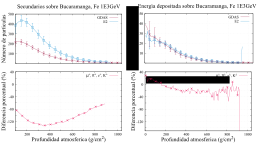
\includegraphics[width=0.8\textwidth]{Figs/fe_1E3.pdf}
\caption[Distribución longitudinal de un núcleo de hierro de $1\cdot 10^{3}$ GeV.]{Distribución longitudinal de un núcleo de hierro de $1\cdot 10^{3} GeV$ que fue simulado 5000 veces, usando la atmósfera predeterminada (línea azul), y usando la atmósfera construida para el mes de abril (línea roja). }
\label{fig:fig27}
\end{figure}

\begin{figure}[htb!]
\centering
\includegraphics[width=0.8\textwidth]{Figs/fe_1E6.pdf}
\caption[Distribución longitudinal de un núcleo de hierro de $1\cdot 10^{6}$ GeV.]{Distribución longitudinal de un núcleo de hierro de $1\cdot 10^{6} GeV$ que fue simulado 1000 veces, usando la atmósfera predeterminada (línea azul), y usando la atmósfera construida para el mes de abril (línea roja). }
\label{fig:fig28}
\end{figure}

\begin{figure}[htb!]
\centering
\includegraphics[width=0.8\textwidth]{Figs/fe_1E8.pdf}
\caption[Distribución longitudinal de un núcleo de hierro de $1\cdot 10^{8}$ GeV.]{Distribución longitudinal de un núcleo de hierro de $1\cdot 10^{3} GeV$ que fue simulado 10 veces, usando la atmósfera predeterminada (línea azul), y usando la atmósfera construida para el mes de abril (línea roja). }
\label{fig:fig29}
\end{figure}

\begin{figure}[htb!]
\centering
\includegraphics[width=0.8\textwidth]{Figs/foton_1E3.pdf}
\caption[Distribución longitudinal de un fotón de $1\cdot 10^{3}$ GeV.]{Distribución longitudinal de un foton de $1\cdot 10^{3} GeV$ que fue simulado 5000 veces, usando la atmósfera predeterminada (línea azul), y usando la atmósfera construida para el mes de abril (línea roja).}
\label{fig:fig30}
\end{figure}

\begin{figure}[htb!]
\centering
\includegraphics[width=0.8\textwidth]{Figs/foton_1E6.pdf}
\caption[Distribución longitudinal de un fotón de $1\cdot 10^{6}$ GeV.]{Distribución longitudinal de un fotón de $1\cdot 10^{6} GeV$ que fue simulado 1000 veces, usando la atmósfera predeterminada (línea azul), y usando la atmósfera construida para el mes de abril (línea roja). }
\label{fig:fig31}
\end{figure}

\begin{figure}[htb!]
\centering
\includegraphics[width=0.8\textwidth]{Figs/foton_1E8.pdf}
\caption[Distribución longitudinal de un fotón de $1\cdot 10^{8}$ GeV.]{Distribución longitudinal de un fotón de $1\cdot 10^{8} GeV$ que fue simulado 10 veces, usando la atmósfera predeterminada (línea azul), y usando la atmósfera construida para el mes de abril (línea roja). }
\label{fig:fig32}
\end{figure}






% ------------------------------------------------------------------------
\end{document}                                          % Fin de documento
% ------------------------------------------------------------------------ 